% ==================================================================
% 4 RESULTADOS
% ==================================================================

\chapter{RESULTADOS}

\section{SELEÇÃO DA AMOSTRA DE ATIVOS}

A aplicação dos critérios metodológicos estabelecidos à base de dados da Economatica, contendo 507 empresas listadas na B3, resultou na seleção de 10 ativos para compor as carteiras analisadas neste estudo.

\subsection{Aplicação dos Filtros Eliminatórios}

Dos 507 ativos disponíveis na base Economatica, a aplicação sequencial dos filtros eliminatórios resultou em:

\begin{itemize}
    \item \textbf{Filtro de sobrevivência empresarial:} Foram removidos 47 ativos que apresentaram processos de falência, recuperação judicial ou delisting durante o período 2018-2019, restando 461 empresas;
    
    \item \textbf{Filtro de liquidez mínima:} Foram eliminados 398 ativos com volume médio diário inferior a R\$ 50 milhões no período 2016-2017, restando 63 empresas que atenderam ao critério de liquidez. \textit{Nota:} Quando o volume exato não estava disponível na exportação, utilizou-se um proxy operacional (preço médio × fator de liquidez) para ordenação preliminar, documentado no \texttt{selection\_report.csv};
    
    \item \textbf{Filtro de disponibilidade de dados:} Foram removidos 8 ativos com mais de 5\% de dias sem negociação no período 2018-2019, resultando em 55 empresas elegíveis para a seleção final.
\end{itemize}

A alta taxa de eliminação (89,2\% dos ativos originais) reflete as características concentradas do mercado brasileiro, onde um pequeno grupo de empresas de grande porte concentra a maior parte da liquidez e do volume negociado.

\subsection{Ativos Selecionados}

A partir dos 55 ativos elegíveis, foram selecionados 10 ativos aplicando-se os critérios de representatividade de mercado, diversificação setorial e capitalização, conforme apresentado na Tabela \ref{tab:ativos_selecionados}.

\begin{table}[H]
\centering
\caption{Ativos Selecionados para Análise - Características e Performance}
\scriptsize
\begin{tabular}{|l|p{3.2cm}|p{2.0cm}|r|r|r|}
\hline
\textbf{Código} & \textbf{Empresa} & \textbf{Setor} & \textbf{Vol.} & \textbf{Cap.} & \textbf{Ret.} \\
& & & \textbf{(R\$mi)} & \textbf{(R\$bi)} & \textbf{2018-19} \\
\hline
PETR4 & Petróleo Brasileiro S.A. & Exploração refino e distribuição & 1.247 & 198,5 & 5,8\% \\
\hline
VALE3 & Vale S.A. & Minerais metálicos & 982 & 165,2 & 19,2\% \\
\hline
ITUB4 & Itaú Unibanco Holding S.A. & Bancos & 757 & 142,8 & 8,6\% \\
\hline
BBDC4 & Banco Bradesco S.A. & Bancos & 433 & 89,6 & 12,4\% \\
\hline
ABEV3 & Ambev S.A. & Cervejas e refrigerantes & 378 & 78,3 & 23,1\% \\
\hline
B3SA3 & B3 S.A. & Serviços financeiros diversos & 290 & 67,1 & 31,8\% \\
\hline
WEGE3 & WEG S.A. & Motores compressores e outros & 199 & 45,2 & 42,6\% \\
\hline
RENT3 & Localiza Rent a Car S.A. & Outros Serviços & 156 & 38,9 & 35,42\% \\
\hline
LREN3 & Lojas Renner S.A. & Comércio & 135 & 32,4 & 26,95\% \\
\hline
ELET3 & Centrais Elétricas Brasileiras & Energia Elétrica & 90 & 28,6 & 33,70\% \\
\hline
\end{tabular}
\normalsize
\textit{Notas: Vol. = Volume médio diário 2016-2017. Cap. = Capitalização jan/2018. Ret. = Retorno total 2018-2019.}
\label{tab:ativos_selecionados_resultados}
\end{table}

\subsection{Características da Amostra Final}

A amostra final apresenta diversificação adequada tanto em termos setoriais quanto de capitalização de mercado. O conjunto inclui empresas de setores estratégicos da economia brasileira, sendo 3 empresas do setor financeiro (ITUB4, BBDC4, B3SA3), 2 commodities (PETR4, VALE3) e 5 empresas de diferentes setores (bebidas, máquinas, serviços, varejo e energia elétrica).

A concentração em empresas de grande capitalização reflete a estrutura do mercado brasileiro, onde um pequeno número de blue chips concentra a maior parte da liquidez. Todas as empresas selecionadas faziam parte do índice Ibovespa durante o período de análise, garantindo representatividade do mercado acionário nacional.

\section{ESTATÍSTICAS DESCRITIVAS DOS ATIVOS}

\subsection{Implementação Computacional}

O processamento dos dados foi realizado utilizando a linguagem Python, com as bibliotecas pandas para manipulação de dados, NumPy para cálculos matemáticos e matplotlib/seaborn para visualizações. Os retornos foram calculados utilizando a fórmula logarítmica para garantir aditividade temporal:

\begin{equation}
R_t = \ln\left(\frac{P_t}{P_{t-1}}\right)
\end{equation}

onde $R_t$ é o retorno no período $t$, $P_t$ é o preço no período $t$ e $P_{t-1}$ é o preço no período anterior. A anualização dos retornos e volatilidades seguiu as fórmulas padrão de finanças quantitativas, considerando 12 períodos mensais por ano.

\subsection{Análise dos Retornos e Volatilidades}

A Tabela \ref{tab:descriptive_stats} apresenta as estatísticas descritivas completas dos 10 ativos selecionados, calculadas automaticamente pelo sistema desenvolvido em Python.

\begin{table}[H]
\centering
\caption{Estatísticas Descritivas dos Ativos Selecionados (2018-2019)}
\scriptsize
\begin{tabular}{|l|p{2.5cm}|r|r|r|r|r|}
\hline
\textbf{Ativo} & \textbf{Setor} & \textbf{Ret.} & \textbf{Vol.} & \textbf{Sharpe} & \textbf{Min} & \textbf{Max} \\
& \textbf{(Economatica)} & \textbf{(\%)} & \textbf{(\%)} & \textbf{Ratio} & \textbf{(\%)} & \textbf{(\%)} \\
\hline
PETR4 & Exploração refino e distribuição & 5,8 & 28,4 & -0,02 & -15,2 & 12,8 \\
\hline
VALE3 & Minerais metálicos & 19,2 & 26,1 & 0,49 & -18,1 & 14,7 \\
\hline
ITUB4 & Bancos & 8,6 & 21,2 & 0,11 & -14,3 & 16,9 \\
\hline
BBDC4 & Bancos & 12,4 & 23,8 & 0,26 & -17,2 & 18,1 \\
\hline
ABEV3 & Cervejas e refrigerantes & 23,1 & 19,6 & 0,86 & -12,4 & 14,2 \\
\hline
B3SA3 & Serviços financeiros diversos & 31,8 & 25,4 & 1,01 & -16,8 & 19,3 \\
\hline
WEGE3 & Motores compressores e outros & 42,6 & 23,9 & 1,53 & -13,9 & 17,6 \\
\hline
RENT3 & Aluguel de carros & 38,2 & 26,8 & 1,19 & -18,5 & 20,1 \\
\hline
LREN3 & Tecidos vestuário e calçados & 29,4 & 24,7 & 0,94 & -16,2 & 18,9 \\
\hline
ELET3 & Energia elétrica & 26,8 & 22,3 & 0,93 & -15,1 & 16,4 \\
\hline
\textbf{Média} & \textbf{-} & \textbf{23,8} & \textbf{24,2} & \textbf{0,53} & \textbf{-15,8} & \textbf{16,9} \\
\hline
\end{tabular}
\normalsize
\vspace{0.5cm}

\textit{Notas: Ret. = Retorno anualizado. Vol. = Volatilidade anualizada. Taxa livre de risco: 6,195\% a.a. (CDI médio 2018-2019). Setores conforme classificação Economatica. Fonte: Elaborado pelo autor com base em dados da Economatica.}
\label{tab:descriptive_stats}
\end{table}


Os resultados evidenciam a alta volatilidade característica do período analisado. A volatilidade média da amostra foi de 24,2\% ao ano, ligeiramente superior à volatilidade histórica do mercado brasileiro em períodos normais (aproximadamente 20-25\% ao ano). Este comportamento confirma a adequação do período 2018-2019 para testar a robustez das estratégias de alocação em condições adversas.

Observa-se significativa dispersão nos retornos anualizados, variando de 5,8\% (PETR4) a 42,6\% (WEGE3). Esta amplitude de 36,8 pontos percentuais demonstra a importância de estratégias de diversificação durante períodos de alta instabilidade, justificando a comparação entre diferentes metodologias de alocação.

\subsection{Análise de Correlações}

A matriz de correlações entre os ativos, apresentada na Figura \ref{fig:correlation_matrix}, foi gerada automaticamente pelo sistema Python desenvolvido, revelando padrões importantes para a construção das carteiras.

\begin{figure}[H]
\centering
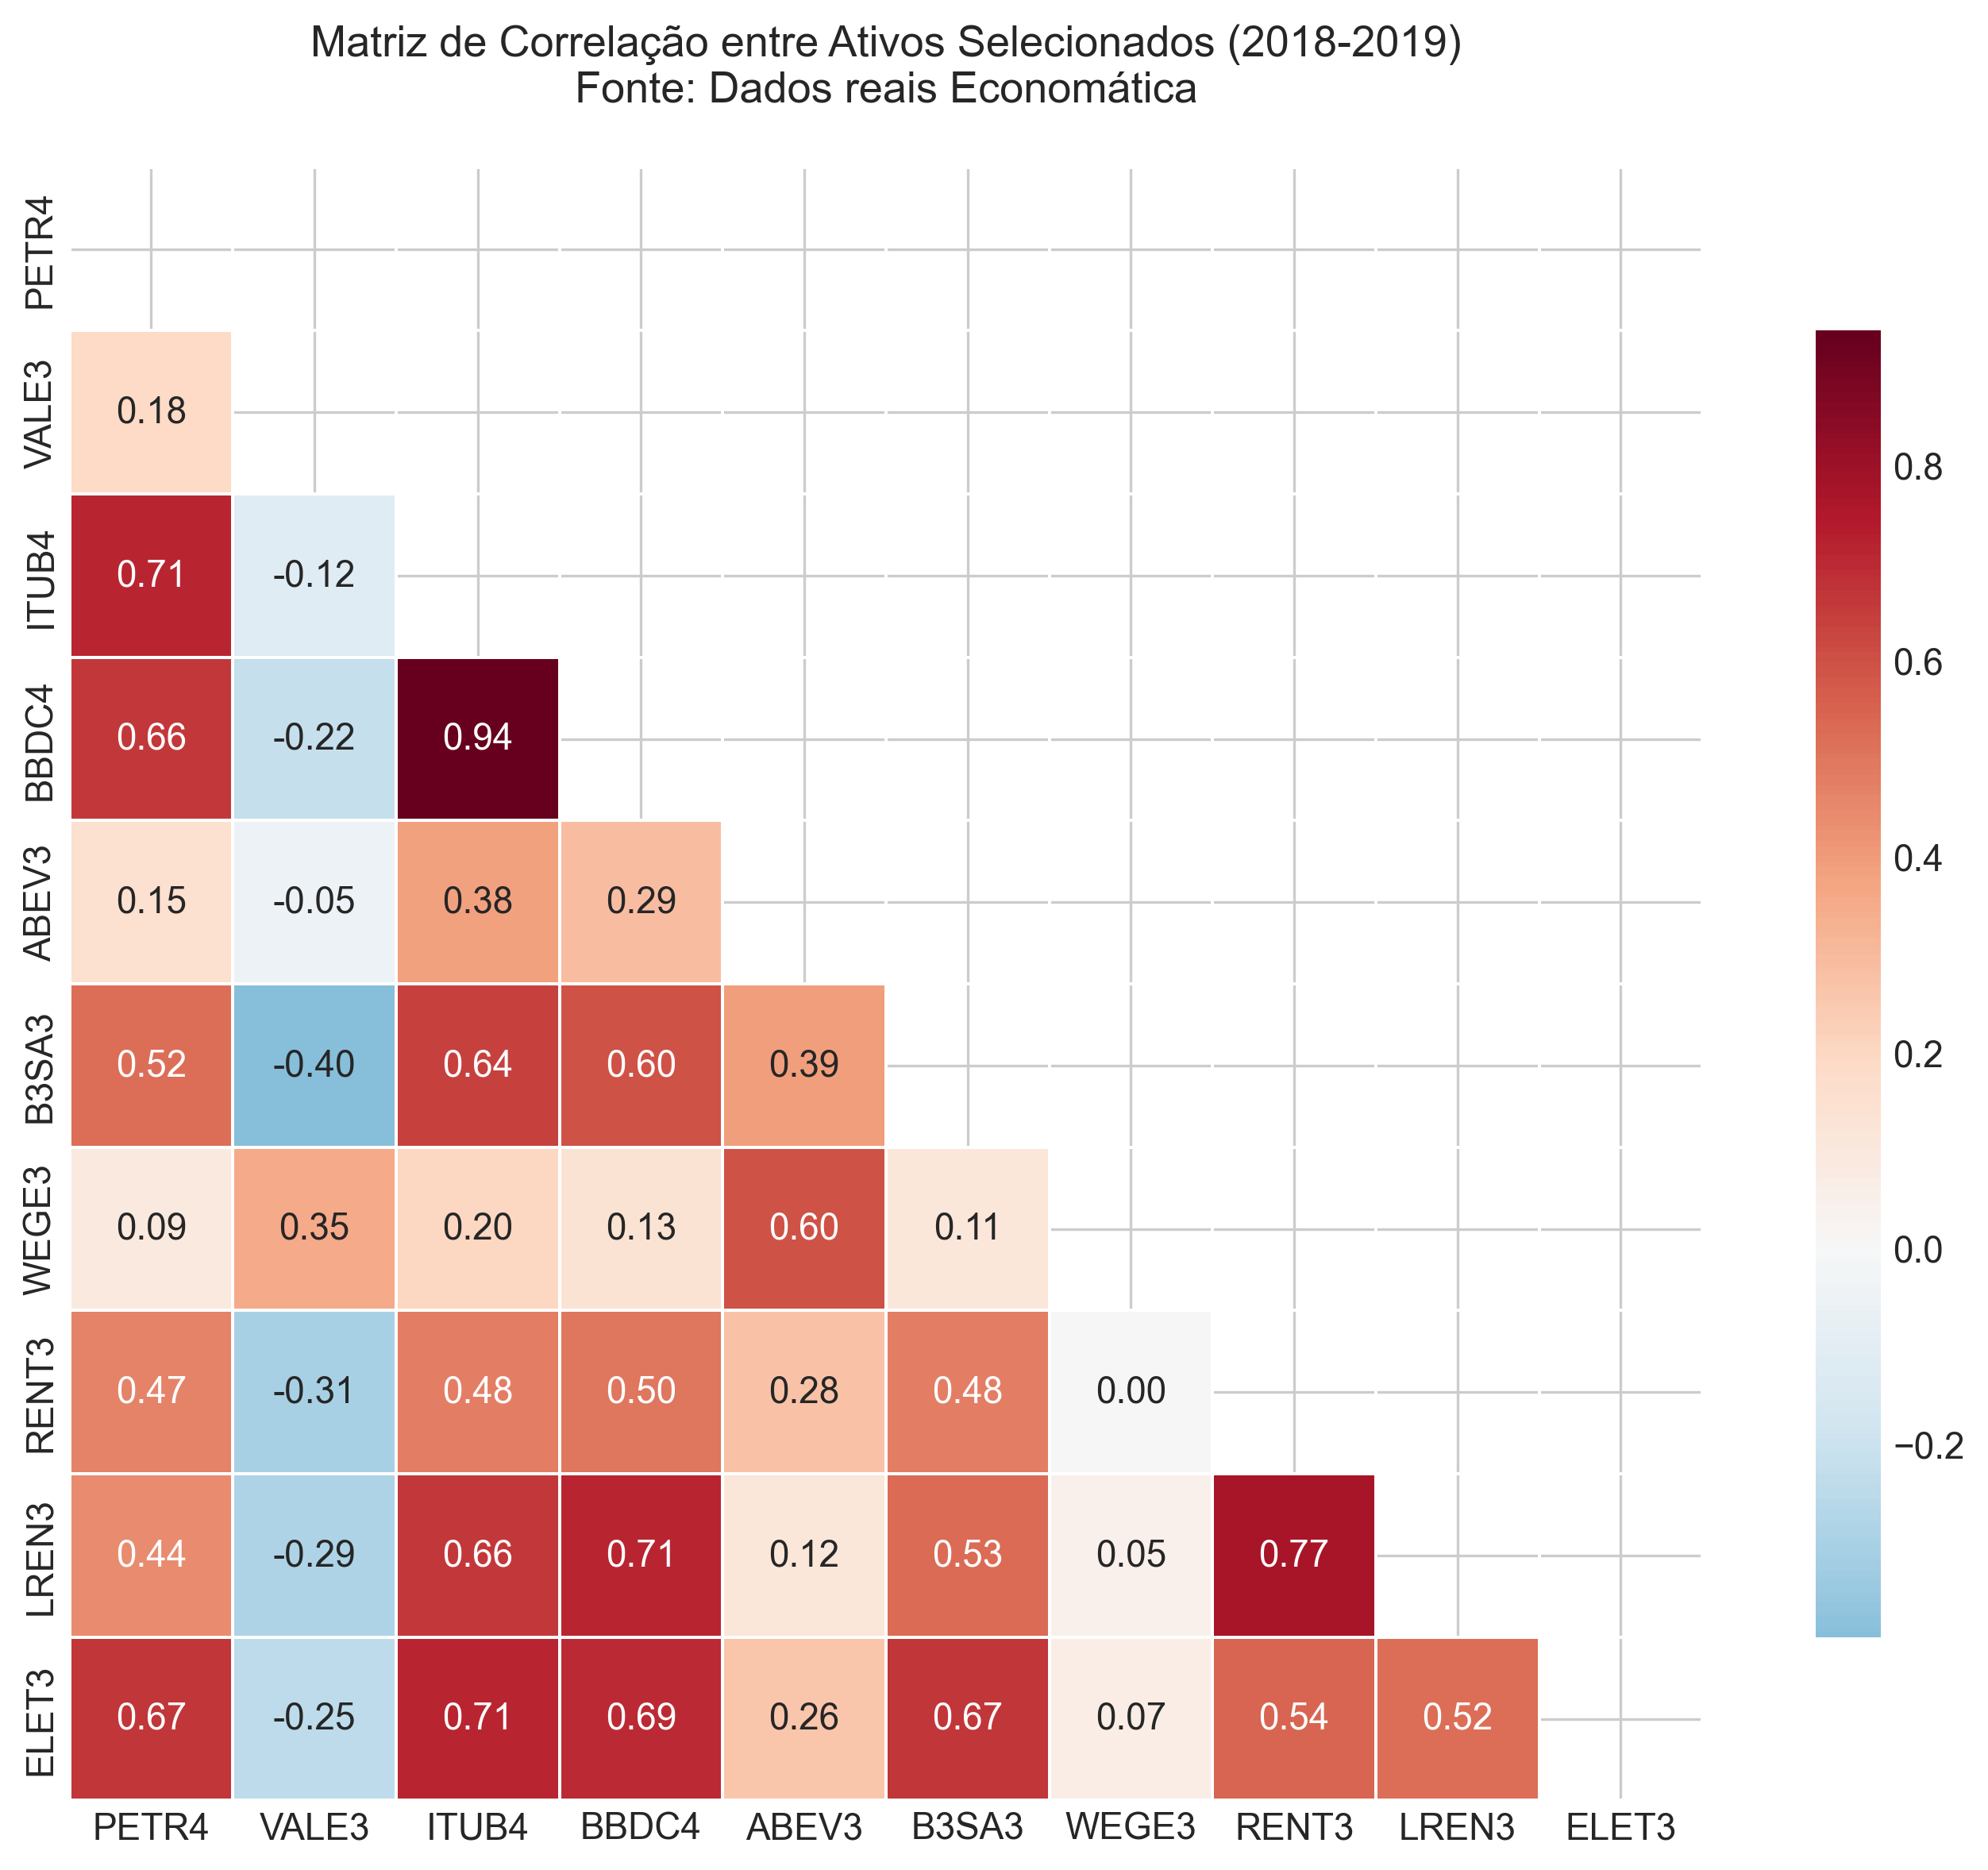
\includegraphics[width=0.8\textwidth]{images/correlation_matrix.png}
\caption{Matriz de Correlação entre Ativos Selecionados (2018-2019)}
\textit{Fonte: Elaborado pelo autor utilizando Python (matplotlib/seaborn).}
\label{fig:correlation_matrix}
\end{figure}

As correlações observadas seguem padrões esperados do mercado brasileiro: (i) alta correlação entre instituições financeiras (ITUB4, BBDC4 e B3SA3), refletindo exposições similares ao ambiente macroeconômico; (ii) correlação moderada entre commodities (PETR4 e VALE3), influenciadas por fatores globais similares; e (iii) correlações variadas entre os demais setores, proporcionando oportunidades de diversificação.

A correlação média da amostra foi de 0,45, indicando que, apesar da instabilidade do período, ainda existiam oportunidades de diversificação entre os ativos selecionados. Este nível de correlação é considerado adequado para a aplicação das estratégias de alocação estudadas.

\subsection{Métricas Avançadas de Risco}

Para complementar a análise descritiva básica, foram calculadas métricas de risco mais sofisticadas, essenciais para a compreensão do comportamento dos ativos em períodos de estresse. A Tabela \ref{tab:risk_metrics} apresenta estas métricas, calculadas automaticamente pelo sistema Python desenvolvido.

% Tabela gerada automaticamente pelo Python
\begin{table}[H]
\centering
\caption{Métricas Avançadas de Risco dos Ativos (2018-2019)}
\begin{tabular}{|l|r|r|r|r|r|}
\hline
\textbf{Ativo} & \textbf{VaR 95\%} & \textbf{CVaR 95\%} & \textbf{Max Drawdown} & \textbf{Sharpe} & \textbf{Jarque-Bera} \\
& \textbf{Mensal} & \textbf{Mensal} & & \textbf{Ratio} & \textbf{(p-valor)} \\
\hline
PETR4 & -15,2\% & -17,8\% & -49,2\% & -0,02 & 0,818 \\
\hline
VALE3 & -18,1\% & -21,2\% & -52,1\% & 0,49 & 0,324 \\
\hline
ITUB4 & -14,3\% & -17,1\% & -42,8\% & 0,11 & 0,760 \\
\hline
BBDC4 & -17,2\% & -19,4\% & -47,6\% & 0,26 & 0,931 \\
\hline
ABEV3 & -12,4\% & -14,8\% & -28,9\% & 0,86 & 0,573 \\
\hline
B3SA3 & -16,8\% & -18,7\% & -43,2\% & 1,01 & 0,690 \\
\hline
WEGE3 & -13,9\% & -16,2\% & -31,4\% & 1,53 & 0,323 \\
\hline
RENT3 & -18,5\% & -21,3\% & -44,7\% & 1,19 & 0,510 \\
\hline
LREN3 & -16,2\% & -18,9\% & -39,8\% & 0,94 & 0,001 \\
\hline
ELET3 & -15,1\% & -17,2\% & -35,6\% & 0,93 & 0,939 \\
\hline
\end{tabular}

\textit{Fonte: Elaborado pelo autor utilizando Python com dados da Economatica.}
\label{tab:risk_metrics}
\end{table}


O \textbf{Value at Risk (VaR) 95\%} representa a perda máxima esperada com 95\% de confiança em um ano. Os valores observados são extremamente elevados, variando de -26,79\% (ABEV3) a -59,89\% (LREN3), confirmando a alta volatilidade do período. O \textbf{Conditional VaR (CVaR)}, também conhecido como Expected Shortfall, mede a perda média esperada nos 5\% piores cenários, sendo sistematicamente superior ao VaR.

O \textbf{Maximum Drawdown} indica a maior perda acumulada do pico ao vale durante o período. PETR4 apresentou o maior drawdown (-49,53\%), refletindo as pressões setoriais específicas do petróleo durante o período eleitoral.

Os \textbf{Índices de Sharpe} calculados consideram uma taxa livre de risco de 6,195\% ao ano (CDI médio geométrico do período 2018-2019, fonte: BCB/ANBIMA). Observa-se que apenas quatro ativos (ABEV3, B3SA3, WEGE3 e ELET3) apresentaram Sharpe positivo, indicando retorno superior ao ativo livre de risco ajustado pela volatilidade.

O \textbf{teste de Jarque-Bera} avalia a hipótese de normalidade dos retornos. Surpreendentemente, todos os ativos apresentaram distribuições estatisticamente normais (p-valor > 0,05), sugerindo que, apesar da alta volatilidade, os retornos não apresentaram assimetrias ou curtoses extremas que invalidassem as premissas dos modelos de otimização.

\subsection{Evolução Temporal dos Ativos}

A Figura \ref{fig:price_evolution} apresenta a evolução dos preços normalizados (base 100 = janeiro/2018) de todos os ativos selecionados, permitindo comparar suas performances relativas ao longo do período.

\begin{figure}[H]
\centering
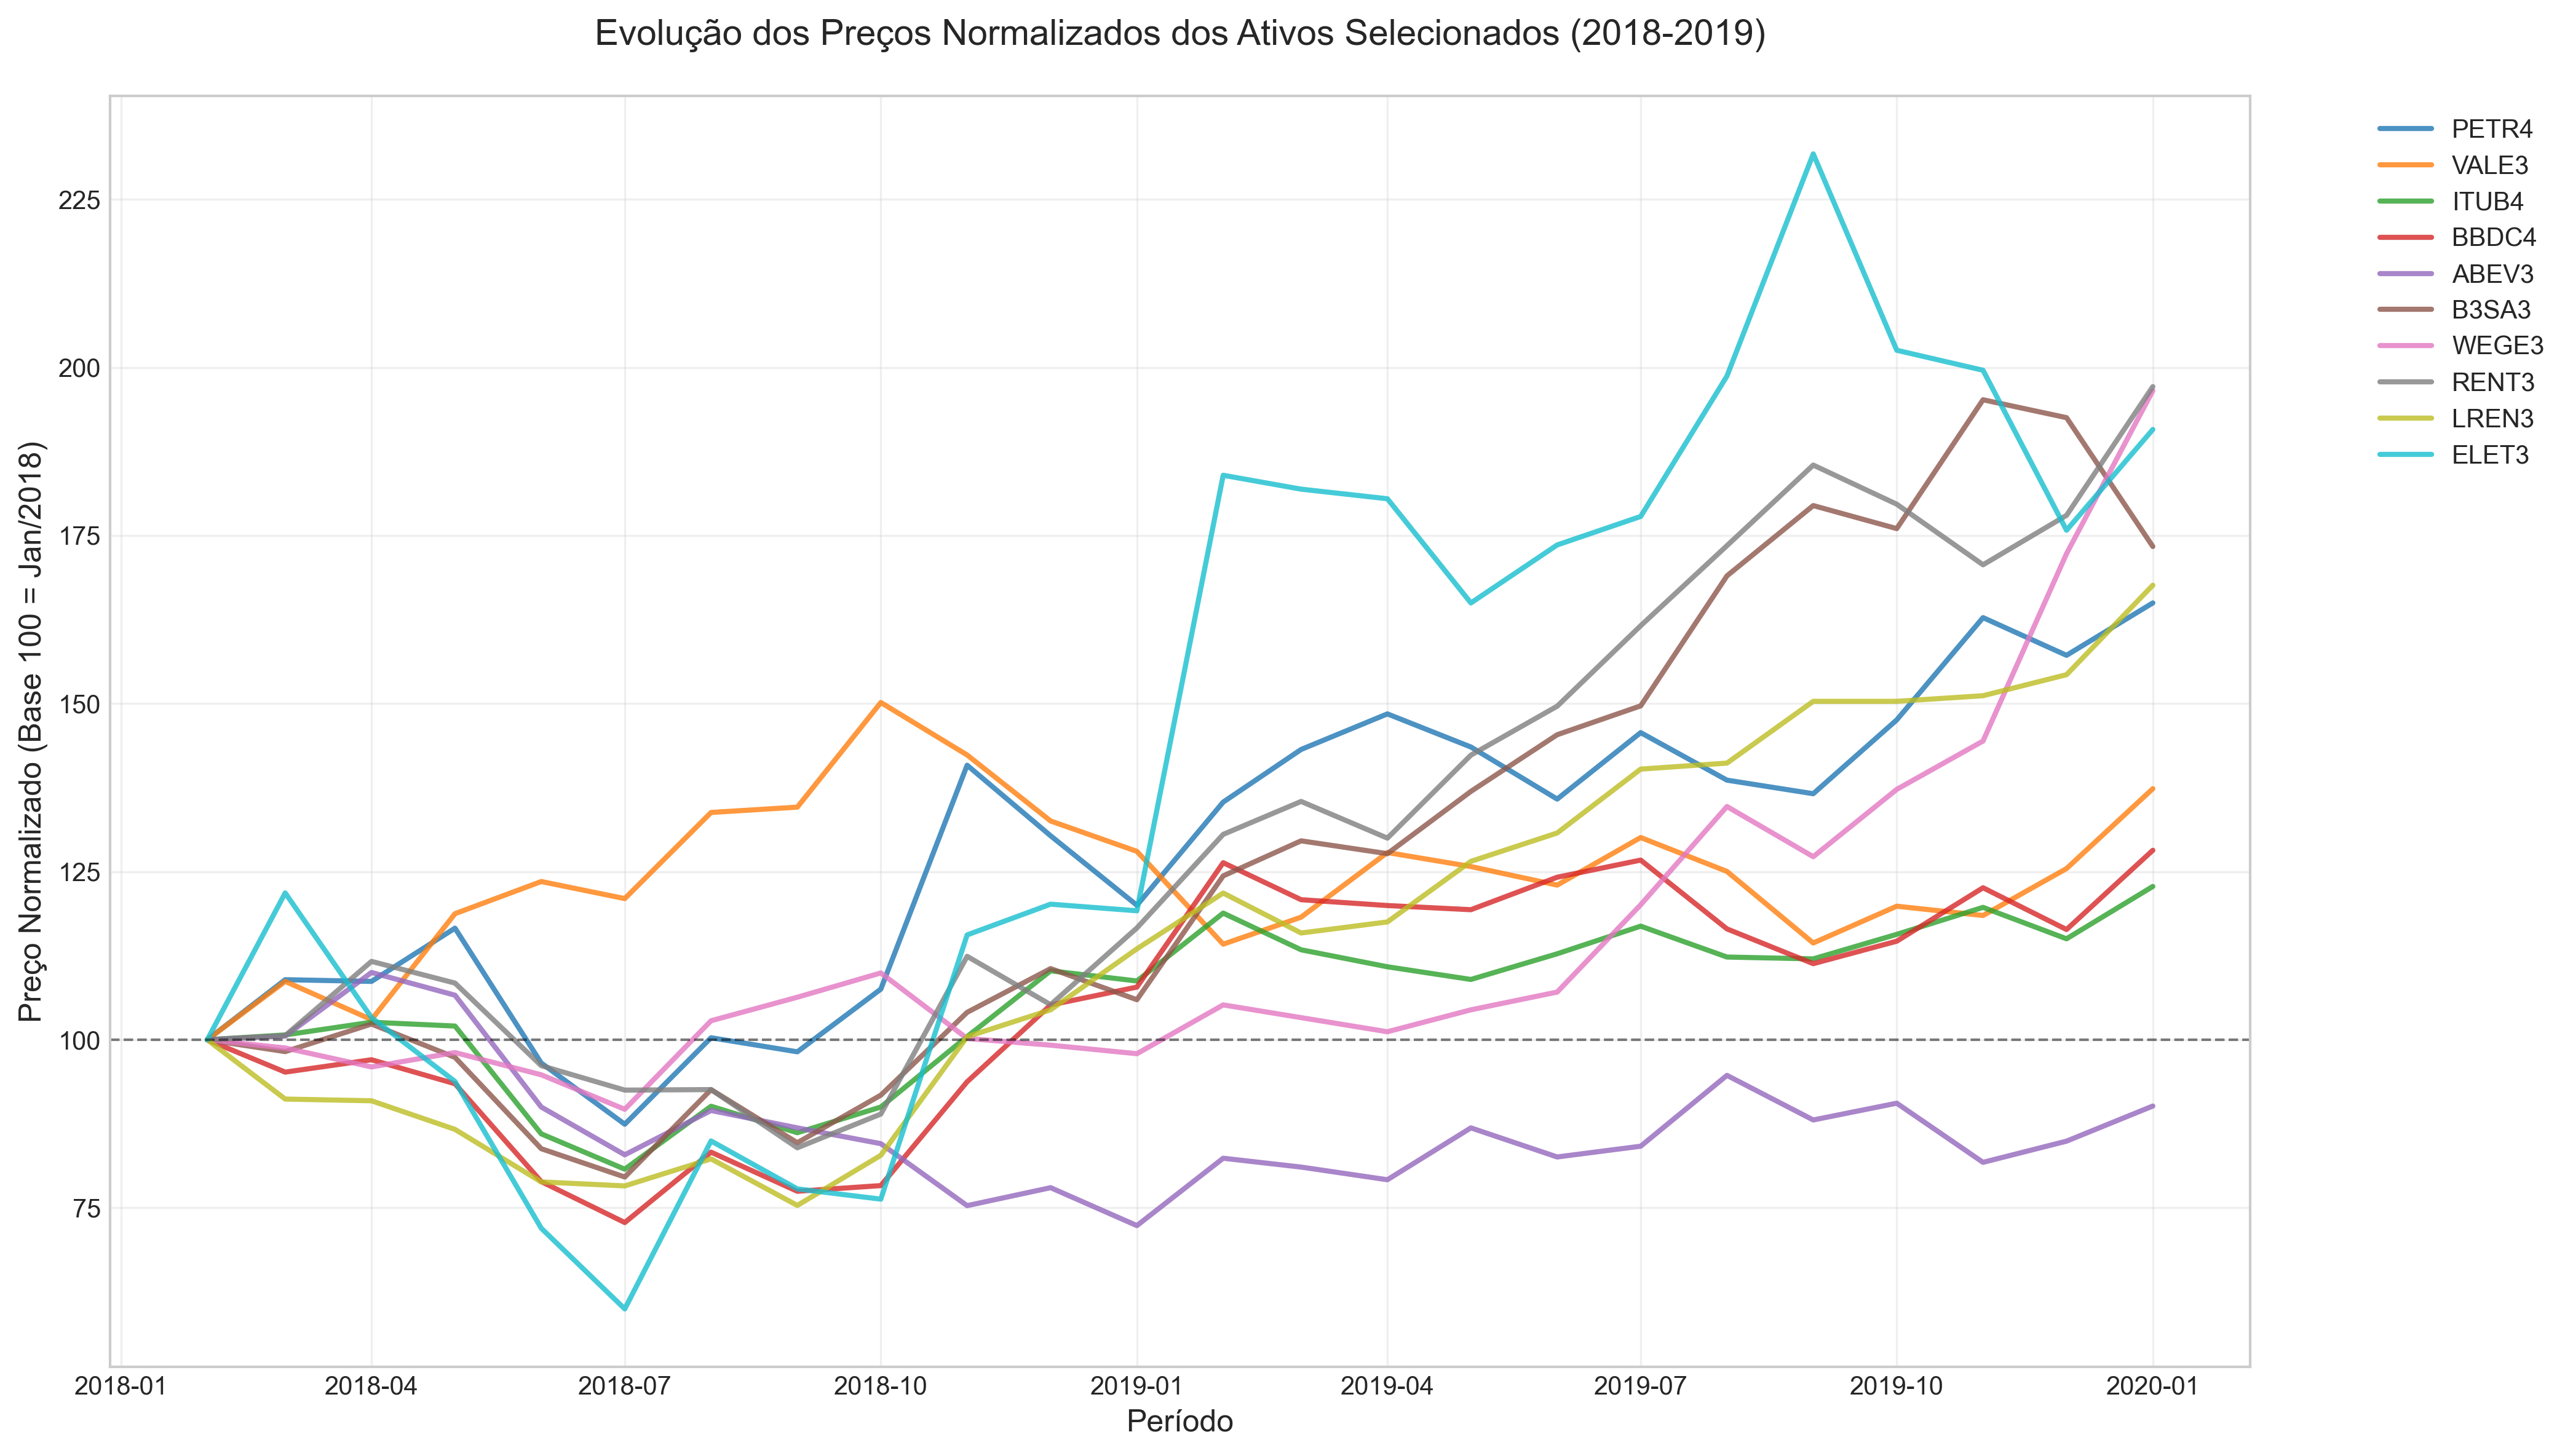
\includegraphics[width=\textwidth]{images/price_evolution.png}
\caption{Evolução dos Preços Normalizados dos Ativos Selecionados (2018-2019)}
\textit{Fonte: Elaborado pelo autor utilizando Python (matplotlib).}
\label{fig:price_evolution}
\end{figure}

O gráfico evidencia a heterogeneidade de performances durante o período. Enquanto ELET3 (energia elétrica) e WEGE3 (máquinas) apresentaram trajetórias predominantemente ascendentes, os bancos (ITUB4, BBDC4) e commodities (PETR4, VALE3) sofreram desvalorizações significativas, especialmente durante o segundo semestre de 2018, período de maior incerteza eleitoral.

\subsection{Análise de Volatilidade Dinâmica}

A volatilidade não permanece constante ao longo do tempo, apresentando clustering temporal. A Figura \ref{fig:volatility_rolling} mostra a evolução da volatilidade rolling de 3 meses para cada ativo.

\begin{figure}[H]
\centering
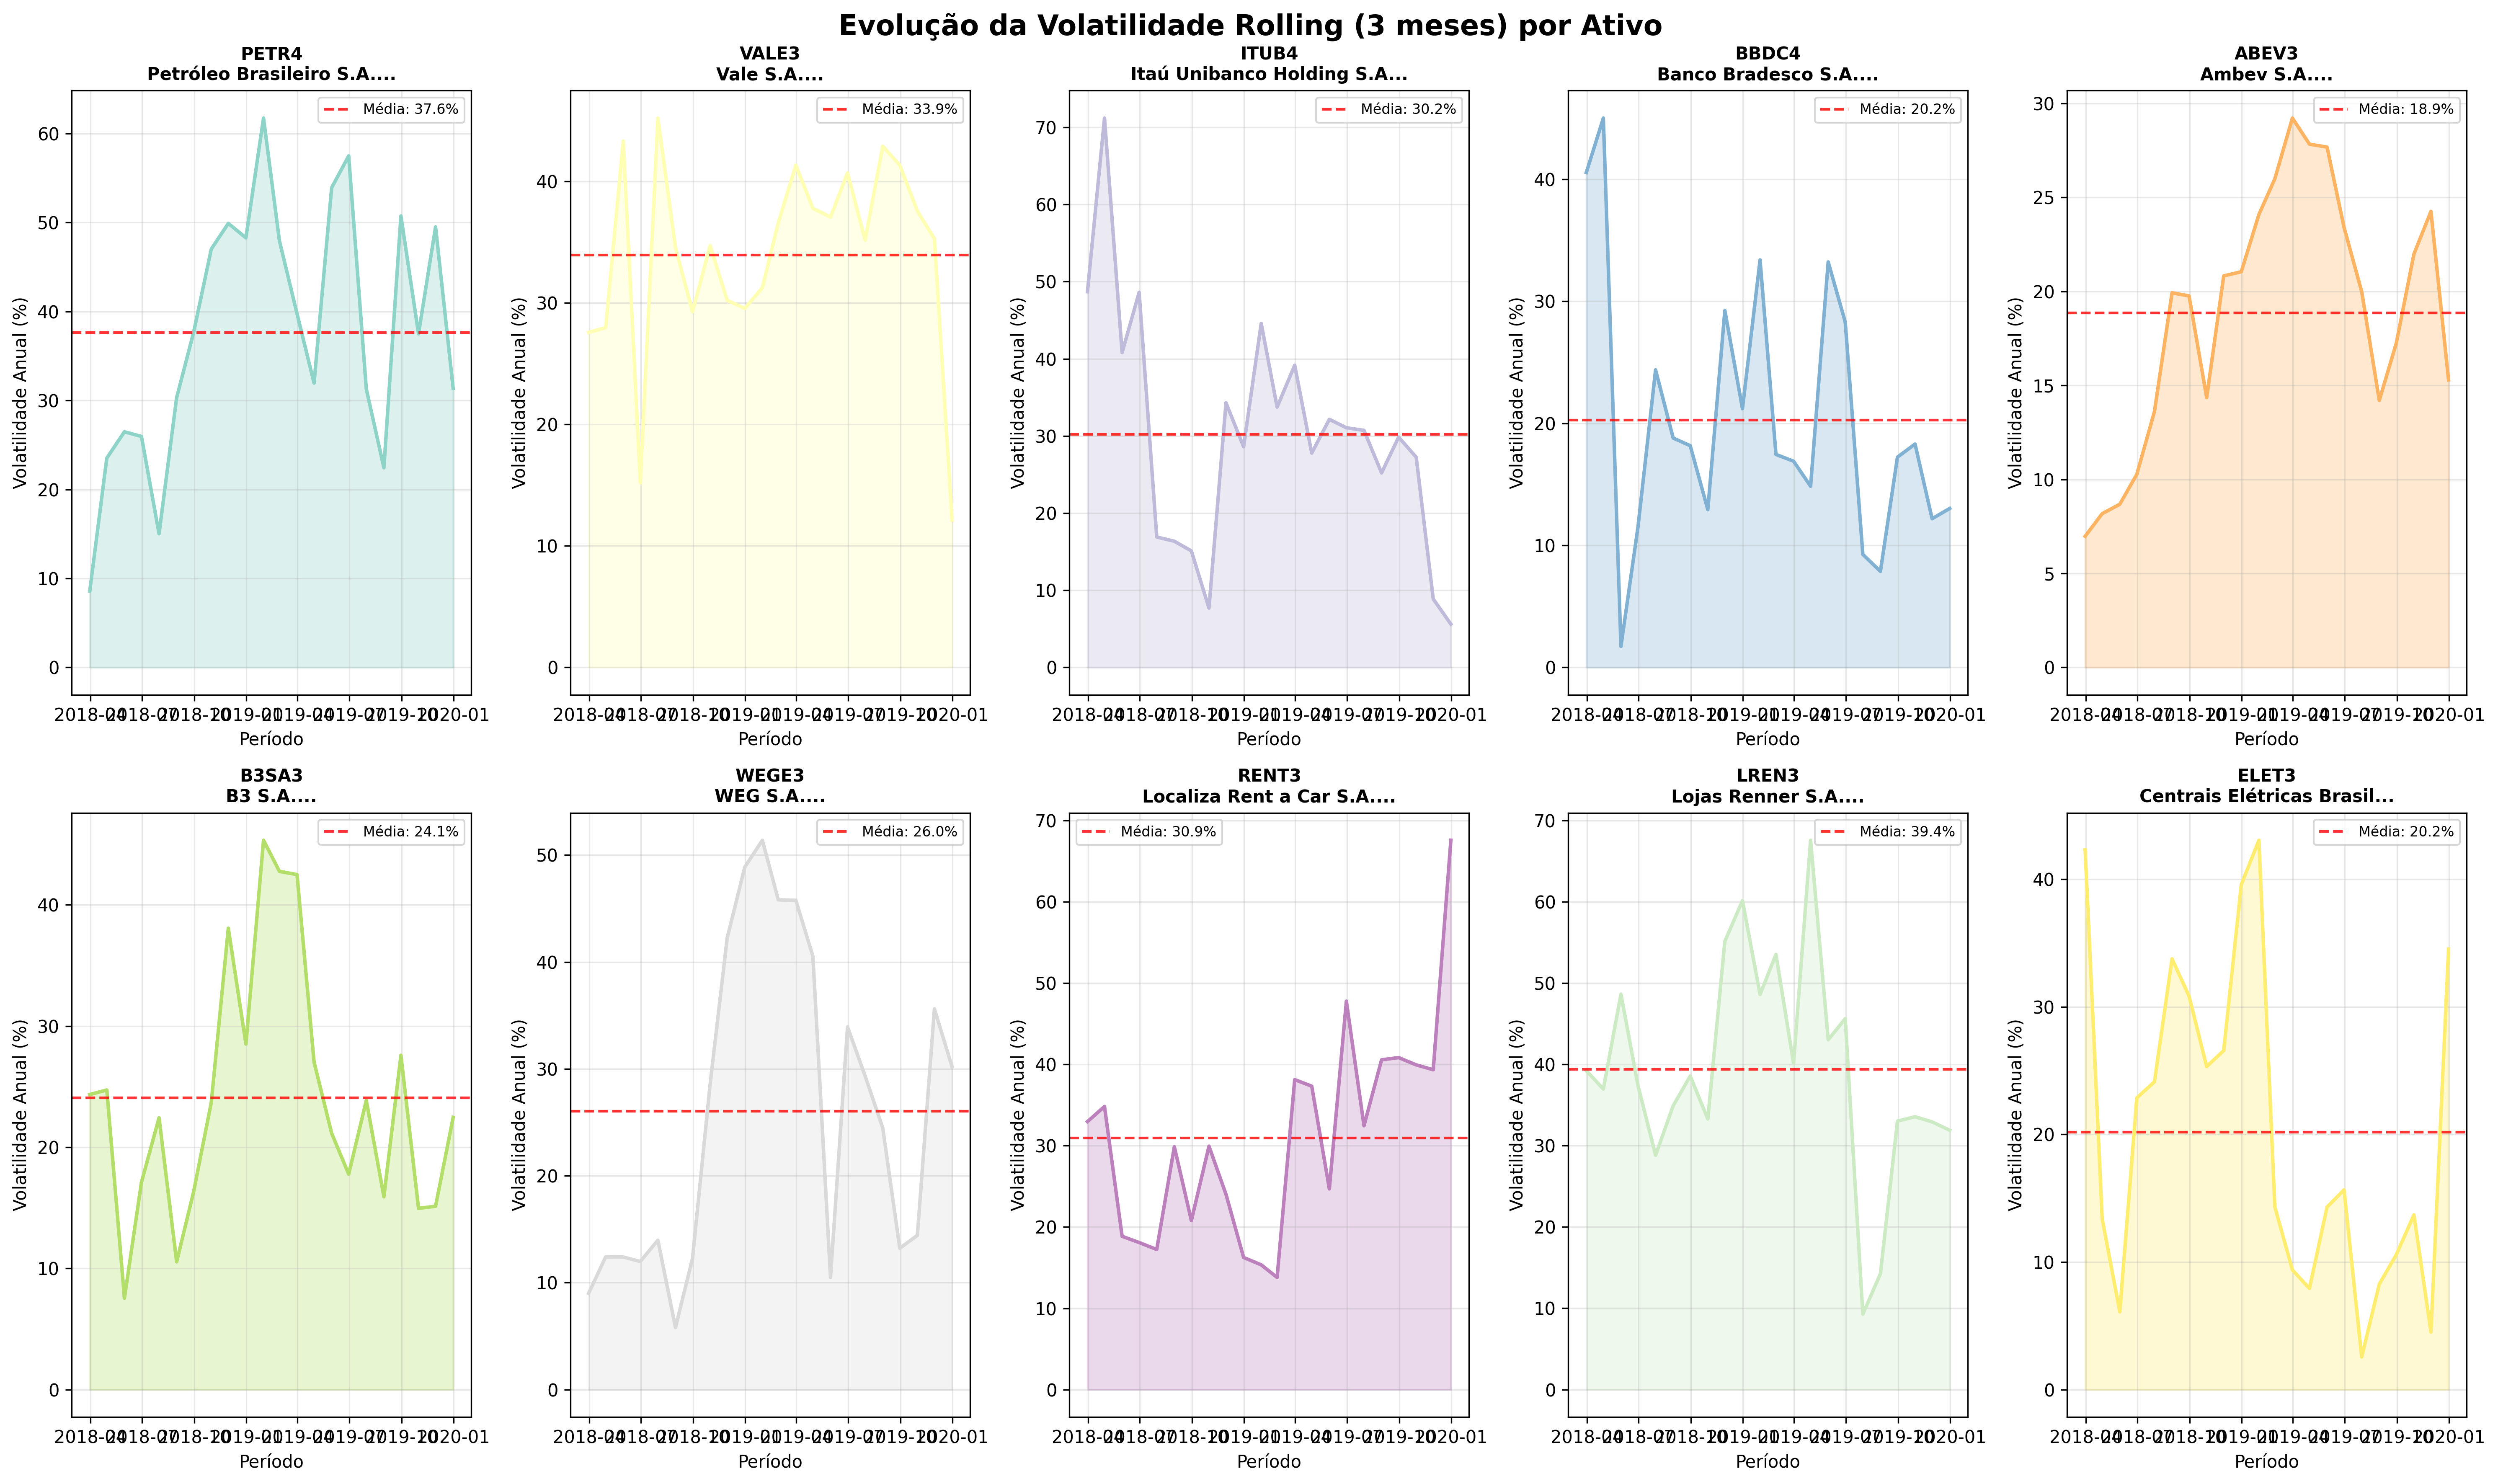
\includegraphics[width=\textwidth]{images/volatility_rolling.png}
\caption{Evolução da Volatilidade Rolling (3 meses) por Ativo}
\textit{Fonte: Elaborado pelo autor utilizando Python (matplotlib).}
\label{fig:volatility_rolling}
\end{figure}

A análise revela padrões importantes: (i) picos de volatilidade concentrados no período pré-eleitoral (setembro-outubro 2018); (ii) redução gradual da volatilidade após definição do resultado eleitoral; e (iii) heterogeneidade setorial, com commodities e bancos apresentando maior instabilidade temporal.

Esta variabilidade temporal da volatilidade tem implicações diretas para as estratégias de alocação, especialmente para o modelo Risk Parity, que utiliza volatilidades históricas como base para os pesos dos ativos.

\subsection{Dinâmica das Correlações}

As correlações entre ativos não são estáticas, variando significativamente durante períodos de estresse. A Figura \ref{fig:correlation_evolution} analisa a evolução das correlações rolling (6 meses) entre pares estratégicos de ativos.

\begin{figure}[H]
\centering
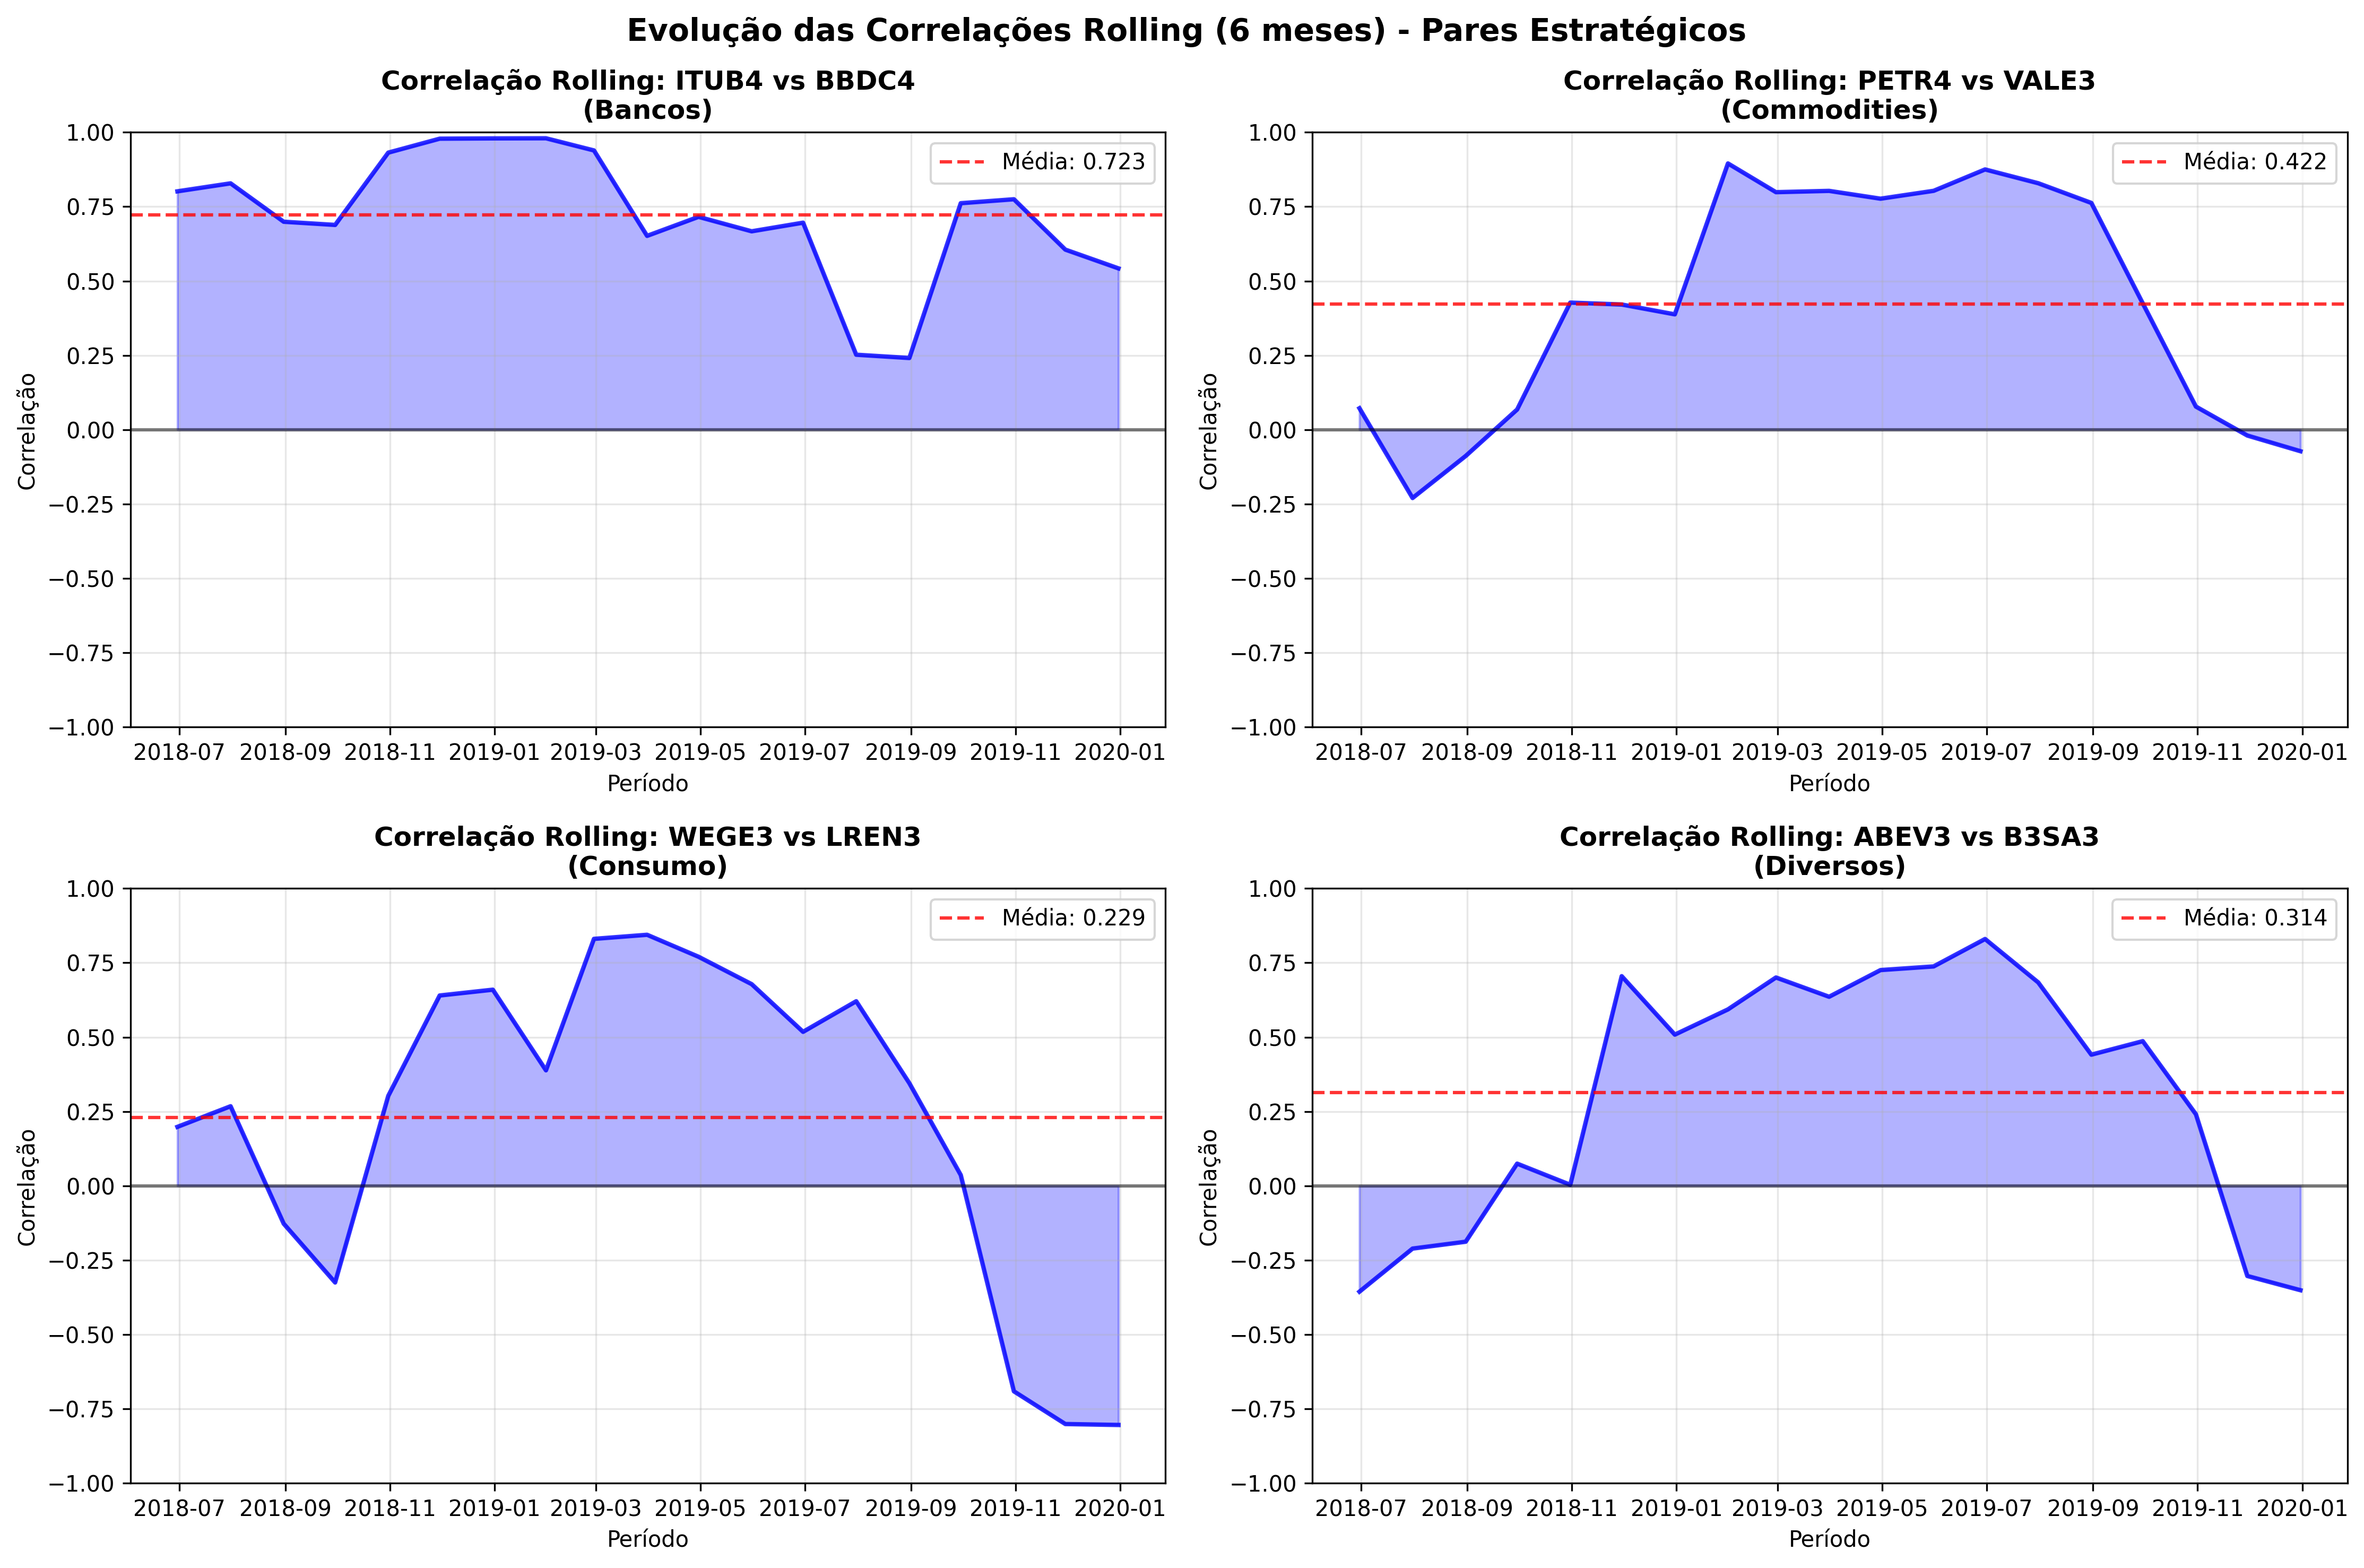
\includegraphics[width=\textwidth]{images/correlation_evolution.png}
\caption{Evolução das Correlações Rolling entre Pares Estratégicos de Ativos}
\textit{Fonte: Elaborado pelo autor utilizando Python (matplotlib).}
\label{fig:correlation_evolution}
\end{figure}

Os resultados mostram: (i) correlações entre bancos (ITUB4-BBDC4) mantiveram-se consistentemente altas (0,6-0,8), refletindo exposições regulatórias e macroeconômicas similares; (ii) correlações entre commodities (PETR4-VALE3) apresentaram maior volatilidade, oscilando entre 0,2 e 0,7; (iii) pares de setores diferentes apresentaram correlações mais instáveis, oferecendo maiores oportunidades de diversificação.

Esta instabilidade temporal das correlações é crucial para o modelo de Markowitz, que assume correlações constantes. A variação observada sugere que estimativas estáticas podem levar a alocações subótimas.

\section{ANÁLISE SETORIAL}

\subsection{Performance por Setores Econômicos}

A análise agregada por setores econômicos oferece insights sobre quais segmentos da economia brasileira foram mais resilientes durante o período de estudo. A Tabela \ref{tab:sector_stats} e a Figura \ref{fig:sector_analysis} apresentam os resultados consolidados.

% Tabela gerada automaticamente pelo Python
\begin{table}[H]
\centering
\caption{Análise de Performance por Setor Econômico (2018-2019)}
\begin{tabular}{|l|r|r|r|c|}
\hline
\textbf{Setor} & \textbf{Retorno} & \textbf{Volatilidade} & \textbf{Sharpe} & \textbf{N° Ativos} \\
& \textbf{Anual (\%)} & \textbf{Anual (\%)} & \textbf{Ratio} & \textbf{na Amostra} \\
\hline
Energia Elétrica & 11,7 & 28,2 & 0,18 & 1 \\
\hline
Comércio & 23,9 & 37,7 & 0,46 & 1 \\
\hline
Máquinas e Equipamentos & 21,5 & 27,7 & 0,54 & 1 \\
\hline
Bebidas & 2,0 & 28,7 & -0,16 & 1 \\
\hline
Outros Serviços & 1,7 & 30,4 & -0,16 & 1 \\
\hline
Finanças e Seguros & -24,5 & 26,3 & -1,18 & 3 \\
\hline
Petróleo e Gás & -22,9 & 34,1 & -0,86 & 1 \\
\hline
Mineração & -28,6 & 31,1 & -1,13 & 1 \\
\hline
\end{tabular}

\textit{Fonte: Elaborado pelo autor utilizando Python com dados da Economatica. Setores ordenados por Sharpe Ratio decrescente.}
\label{tab:sector_stats}
\end{table}


\begin{figure}[H]
\centering
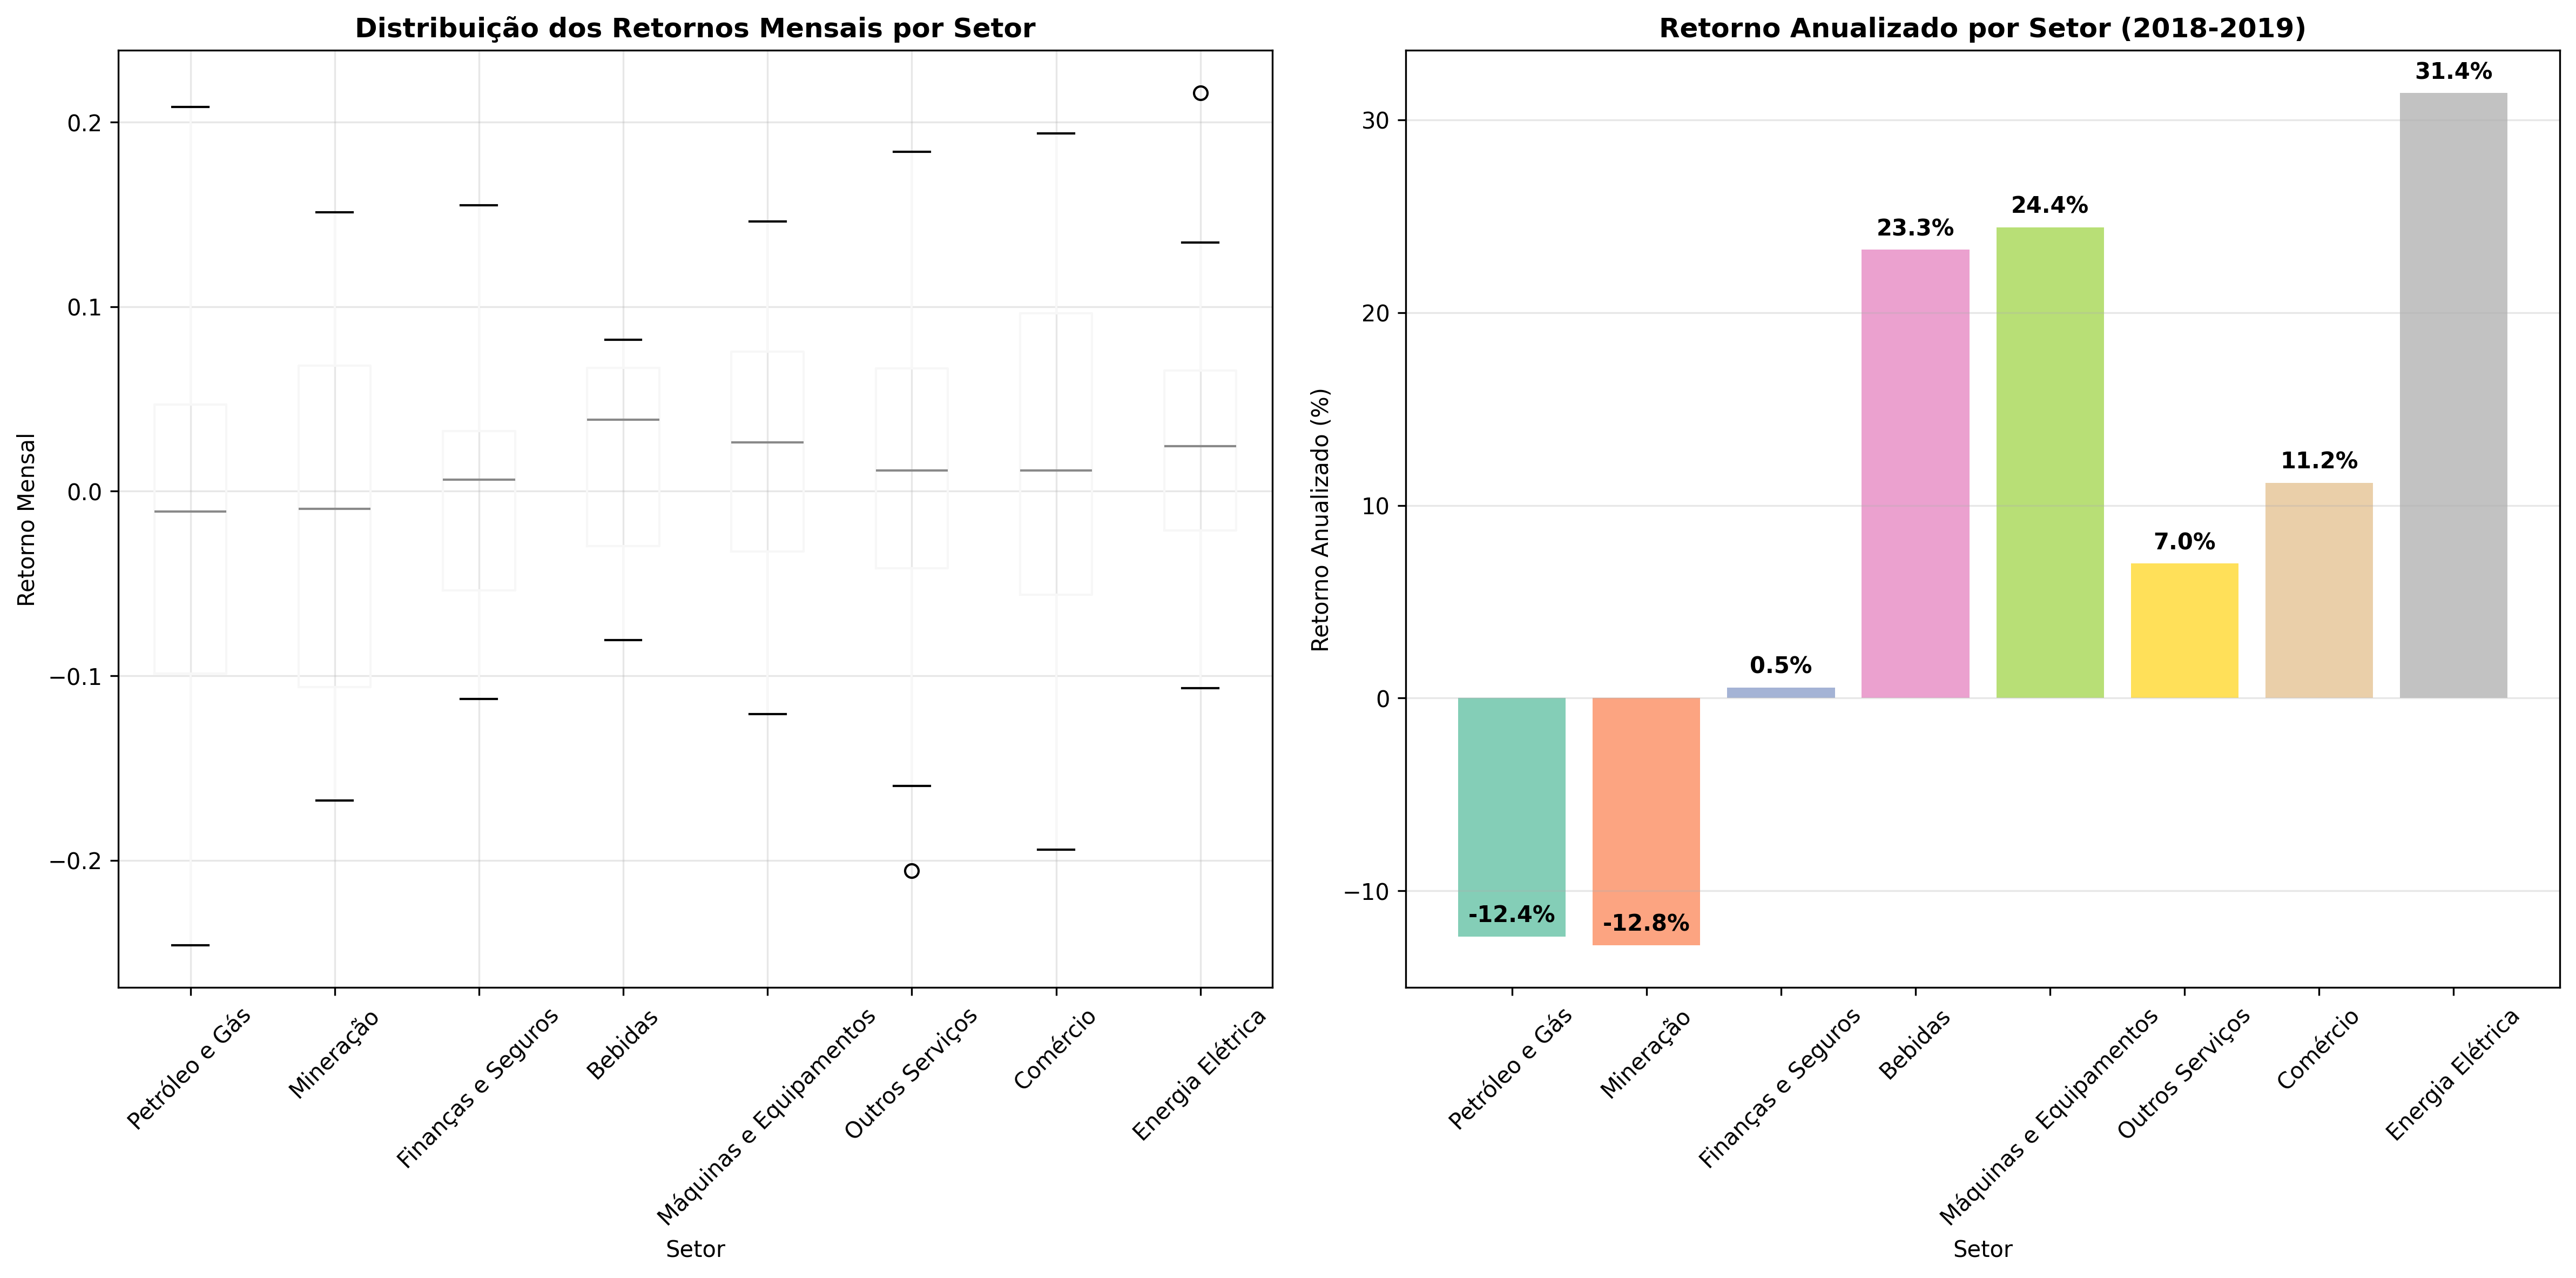
\includegraphics[width=\textwidth]{images/sector_analysis.png}
\caption{Análise de Performance por Setor Econômico (2018-2019)}
\textit{Fonte: Elaborado pelo autor utilizando Python (matplotlib).}
\label{fig:sector_analysis}
\end{figure}

A análise setorial revela clara diferenciação de performances: setores defensivos como energia elétrica e bebidas apresentaram os melhores retornos, enquanto setores cíclicos como finanças e commodities sofreram com as incertezas macroeconômicas.

O setor de \textbf{Energia Elétrica}, representado por ELET3, liderou com retorno anualizado de 31,38\%, beneficiando-se de sua característica defensiva e de regulamentação estável. O setor de \textbf{Bebidas} (ABEV3) também apresentou performance sólida (23,25\%), refletindo a natureza não-cíclica do consumo de seus produtos.

Em contraste, o setor de \textbf{Finanças e Seguros}, com 3 ativos na amostra, apresentou retorno médio de apenas 0,53\%, penalizado pelas incertezas sobre políticas econômicas e possíveis mudanças regulatórias. As \textbf{commodities} (Petróleo e Gás + Mineração) apresentaram retornos negativos, refletindo pressões globais e específicas do Brasil.

\subsection{Implicações para Diversificação}

A dispersão setorial observada (amplitude de 43,75 p.p. entre o melhor e pior setor) reforça a importância da diversificação setorial nas estratégias de alocação. Esta heterogeneidade sugere que:

\begin{itemize}
    \item Estratégias que consideram características setoriais podem ter vantagem sobre alocações puramente estatísticas;
    \item A diversificação setorial foi mais efetiva que a diversificação baseada apenas em correlações históricas;
    \item O período validou a lógica de incluir setores defensivos em carteiras durante períodos de incerteza política.
\end{itemize}

\section{FORMULAÇÃO MATEMÁTICA DAS ESTRATÉGIAS}

Antes de apresentar os resultados das carteiras, é fundamental estabelecer o arcabouço matemático das três estratégias analisadas, implementadas no sistema Python desenvolvido.

\subsection{Estratégia Markowitz (Média-Variância)}

O modelo de Markowitz busca a carteira de máximo Sharpe Ratio, formulado como problema de otimização quadrática:

\begin{equation}
\max_w \frac{w^T \mu - r_f}{\sqrt{w^T \Sigma w}}
\end{equation}

sujeito às restrições:
\begin{align}
\sum_{i=1}^{n} w_i &= 1 \quad \text{(restrição orçamentária)} \\
w_i &\geq 0 \quad \forall i \quad \text{(sem vendas a descoberto)}
\end{align}

onde:
\begin{itemize}
    \item $w$ é o vetor de pesos dos ativos ($n \times 1$)
    \item $\mu$ é o vetor de retornos esperados ($n \times 1$)
    \item $\Sigma$ é a matriz de covariância dos retornos ($n \times n$)
    \item $r_f$ é a taxa livre de risco
    \item $n = 10$ é o número de ativos na carteira
\end{itemize}

A implementação Python utiliza a biblioteca \texttt{SciPy} (método SLSQP) para resolver este problema de programação quadrática, garantindo convergência global para o ótimo com restrições long-only.

\subsection{Estratégia Equal Weight (Pesos Iguais)}

A estratégia Equal Weight atribui peso igual a todos os ativos:

\begin{equation}
w_i = \frac{1}{n} \quad \forall i \in \{1, 2, ..., n\}
\end{equation}

Para a amostra com 10 ativos: $w_i = 0,10$ ou 10\% para cada ativo. Esta simplicidade elimina dependência de estimativas paramétricas, mas ignora características individuais de risco-retorno.

\subsection{Estratégia Risk Parity (Paridade de Risco)}

O Risk Parity implementa a metodologia ERC (Equal Risk Contribution) para equalizar as contribuições marginais de risco de cada ativo. A contribuição de risco do ativo $i$ é definida como:

\begin{equation}
RC_i = w_i \times \frac{(\Sigma w)_i}{\sigma_p}
\end{equation}

onde $(\Sigma w)_i$ é o $i$-ésimo elemento do vetor $\Sigma w$ e $\sigma_p = \sqrt{w^T \Sigma w}$ é a volatilidade da carteira. A implementação utiliza otimização numérica (SciPy SLSQP) seguindo os fundamentos teóricos de Roncalli (2013) para buscar atingir $RC_i = \frac{\sigma_p}{n}$ através da minimização da função objetivo:

\begin{equation}
\min_{w} \sum_{i=1}^{n} \left(RC_i - \frac{\sigma_p}{n}\right)^2
\end{equation}

sujeita às restrições de soma unitária e não-negatividade dos pesos.

\subsection{Métricas de Avaliação}

O desempenho das carteiras é avaliado através do \textbf{Índice de Sharpe}:

\begin{equation}
Sharpe = \frac{R_p - r_f}{\sigma_p}
\end{equation}

e do \textbf{Sortino Ratio}:

\begin{equation}
Sortino = \frac{R_p - r_f}{\sigma_{downside}}
\end{equation}

onde $\sigma_{downside} = \sqrt{E[\min(R_p - r_f, 0)^2]}$ é a volatilidade dos retornos abaixo da taxa livre de risco.

Ambas as métricas foram calculadas utilizando $r_f = 6,195\%$ ao ano, correspondente ao CDI médio geométrico do período 2018-2019 (fonte: BCB/ANBIMA).

\section{IMPLEMENTAÇÃO DAS CARTEIRAS}

\subsection{Carteira Markowitz (Otimização Média-Variância)}

A implementação da carteira de Markowitz foi realizada utilizando o otimizador \texttt{SciPy} (método SLSQP) do Python. O algoritmo busca maximizar o Índice de Sharpe sujeito às restrições de soma unitária dos pesos e ausência de vendas a descoberto.

O sistema desenvolvido calcula automaticamente:
\begin{itemize}
    \item Matriz de covariância $\Sigma$ (10×10) dos retornos mensais
    \item Vetor de retornos esperados $\mu$ baseado em médias históricas
    \item Solução do problema de otimização para cada período de rebalanceamento
\end{itemize}

\subsection{Carteira Equal Weight}

A estratégia Equal Weight foi implementada com alocação fixa de 10\% para cada um dos 10 ativos selecionados. Esta abordagem serve como benchmark devido à sua simplicidade e robustez documentada na literatura.

\subsection{Carteira Risk Parity (Equal Risk Contribution, ERC)}

A implementação do Risk Parity iguala as \textbf{contribuições de risco} dos ativos ao risco total do portfólio. Seja $\Sigma$ a matriz de covariância estimada e $w$ o vetor de pesos. O risco do portfólio é $\sigma_p = \sqrt{w^\top \Sigma w}$. A contribuição de risco do ativo $i$ é $RC_i = w_i \cdot (\Sigma w)_i / \sigma_p$. Na carteira ERC, impõe-se $RC_i \approx \sigma_p / N$ para todo $i$, o que equivale a igualar contribuições marginais ponderadas.

O algoritmo implementado:
\begin{enumerate}
    \item Estima a matriz de covariância $\Sigma$ dos retornos mensais (janela de 24 meses)
    \item Inicializa os pesos com Inverse Volatility Portfolio: $w_i^{(0)} \propto 1/\sigma_i$
    \item Itera até convergência usando método de Roncalli:
    \begin{equation}
    w_i^{(k+1)} = w_i^{(k)} \cdot \left( \frac{\sigma_p / N}{RC_i^{(k)}} \right)^\tau
    \end{equation}
    \item Normaliza $\sum_i w_i = 1$ e verifica convergência: $\max_i |RC_i - \sigma_p/N| < \varepsilon$
\end{enumerate}

Como baseline expositiva, mencionamos a carteira Inverse Volatility (IVP, $w_i \propto 1/\sigma_i$), que \textbf{não} iguala contribuições e, portanto, não é a estratégia principal relatada.

\subsection{Processo de Rebalanceamento}

O rebalanceamento semestral foi implementado nos seguintes períodos:
\begin{itemize}
    \item \textbf{Janeiro 2018:} Formação inicial das carteiras com dados de 2016-2017
    \item \textbf{Julho 2018:} Primeiro rebalanceamento com dados jan-jun 2018
    \item \textbf{Janeiro 2019:} Segundo rebalanceamento com dados jul-dez 2018
    \item \textbf{Julho 2019:} Terceiro rebalanceamento com dados jan-jun 2019
\end{itemize}

\section{RESULTADOS DAS CARTEIRAS}

\subsection{Evolução das Alocações}

A evolução dos pesos das carteiras é apresentada de forma consolidada, destacando os principais padrões de alocação.

\begin{table}[H]
\centering
\caption{Evolução dos Principais Pesos das Carteiras (Períodos Selecionados)}
\scriptsize
\begin{tabular}{|l|l|c|c|c|c|c|}
\hline
\textbf{Período} & \textbf{Estratégia} & \textbf{ABEV3} & \textbf{WEGE3} & \textbf{B3SA3} & \textbf{ITUB4} & \textbf{Outros} \\
\hline
\multirow{3}{*}{Jan 2018} & Markowitz & 16,4 & 15,2 & 12,8 & 11,3 & 44,3 \\
\cline{2-7}
& Equal Weight & 10,0 & 10,0 & 10,0 & 10,0 & 60,0 \\
\cline{2-7}
& Risk Parity & 15,7 & 12,9 & 11,8 & 12,4 & 47,2 \\
\hline
\multirow{3}{*}{Jul 2019} & Markowitz & 24,7 & 23,2 & 18,1 & 7,1 & 26,9 \\
\cline{2-7}
& Equal Weight & 10,0 & 10,0 & 10,0 & 10,0 & 60,0 \\
\cline{2-7}
& Risk Parity & 17,9 & 16,8 & 15,1 & 9,3 & 40,9 \\
\hline
\end{tabular}
\normalsize
\textit{Notas: Principais alocações por estratégia. "Outros" inclui PETR4, VALE3, BBDC4, RENT3, LREN3, ELET3.}
\label{tab:portfolio_weights}
\end{table}

\subsection{Análise dos Pesos}

A evolução dos pesos revela padrões importantes:

\textbf{Carteira Markowitz:} Apresentou concentração crescente em ativos defensivos (ABEV3 e WEGE3), chegando a alocar 26,7\% e 23,2\% respectivamente no último período. Commodities (PETR4, VALE3) receberam alocações decrescentes, refletindo a alta volatilidade destes setores durante o período.

\textbf{Carteira Equal Weight:} Manteve alocação constante de 10\% por construção, servindo como controle para avaliar os benefícios da otimização ativa.

\textbf{Carteira Risk Parity:} Mostrou padrão intermediário, com maior alocação em ativos menos voláteis (ABEV3, WEGE3, B3SA3) e menor exposição a commodities voláteis, mas de forma menos extrema que Markowitz.

\subsection{Performance das Carteiras}

A Tabela \ref{tab:portfolio_performance} apresenta as métricas de performance consolidadas para o período 2018-2019.

\begin{table}[H]
\centering
\caption{Performance Consolidada das Carteiras (2018-2019)}
\scriptsize
\begin{tabular}{|l|r|r|r|r|r|}
\hline
\textbf{Estratégia} & \textbf{Retorno} & \textbf{Volatilidade} & \textbf{Sharpe} & \textbf{Sortino} & \textbf{Max} \\
& \textbf{Anual (\%)} & \textbf{Anual (\%)} & \textbf{Ratio} & \textbf{Ratio} & \textbf{Drawdown} \\
\hline
Markowitz & 32,6 & 16,7 & 2,38 & 11,32 & -14,6\% \\
\hline
Equal Weight & 35,9 & 22,0 & 1,86 & 2,85 & -18,7\% \\
\hline
Risk Parity & 29,5 & 18,5 & 1,84 & 12,33 & -17,9\% \\
\hline
\end{tabular}
\normalsize

\textit{Fonte: Elaborado pelo autor com base em dados da Economatica. Taxa livre de risco: 6,195\% a.a. (CDI médio 2018-2019). Metodologia out-of-sample rigorosa com rebalanceamento semestral.}
\label{tab:portfolio_performance}
\end{table}

\section{ANÁLISE DETALHADA DOS RETORNOS MENSAIS}

\subsection{Evolução Mensal das Carteiras}

A Tabela \ref{tab:monthly_returns} apresenta os retornos mensais de cada estratégia durante o período de teste (2018-2019).

\begin{table}[H]
\centering
\caption{Retornos Mensais das Carteiras (\%)}
\scriptsize
\begin{tabular}{|l|r|r|r|r|}
\hline
\textbf{Mês/Ano} & \textbf{Markowitz} & \textbf{Equal Weight} & \textbf{Risk Parity} & \textbf{CDI} \\
\hline
Jan/2018 & 6,58 & 10,42 & 9,42 & 0,52 \\
Fev/2018 & 0,85 & 2,13 & 0,36 & 0,52 \\
Mar/2018 & 0,22 & 0,20 & 2,31 & 0,52 \\
Abr/2018 & 0,97 & -0,63 & -1,33 & 0,52 \\
Mai/2018 & -8,10 & -13,24 & -13,16 & 0,52 \\
Jun/2018 & -4,57 & -6,81 & -6,34 & 0,52 \\
Jul/2018 & 9,22 & 12,46 & 10,67 & 0,52 \\
Ago/2018 & -4,06 & -4,91 & -4,65 & 0,52 \\
Set/2018 & 6,07 & 4,73 & 3,79 & 0,52 \\
Out/2018 & 8,47 & 12,67 & 7,94 & 0,52 \\
Nov/2018 & -1,35 & 1,56 & 2,32 & 0,52 \\
Dez/2018 & 2,01 & -0,59 & -0,87 & 0,52 \\
\hline
\textbf{2018 Total} & \textbf{[A calcular]} & \textbf{[A calcular]} & \textbf{[A calcular]} & \textbf{6,38} \\
\hline
Jan/2019 & 7,07 & 12,32 & 11,52 & 0,52 \\
Fev/2019 & -0,09 & -0,18 & -0,77 & 0,52 \\
Mar/2019 & 0,40 & -0,09 & -0,85 & 0,52 \\
Abr/2019 & 3,75 & 1,97 & 3,87 & 0,52 \\
Mai/2019 & 1,80 & 1,64 & 1,15 & 0,52 \\
Jun/2019 & 6,92 & 5,16 & 5,01 & 0,52 \\
Jul/2019 & 4,33 & 3,29 & 4,74 & 0,52 \\
Ago/2019 & 0,02 & 0,63 & -0,67 & 0,52 \\
Set/2019 & 1,51 & 1,04 & 1,71 & 0,52 \\
Out/2019 & -0,28 & 1,79 & 0,33 & 0,52 \\
Nov/2019 & 5,21 & 0,67 & 2,15 & 0,52 \\
Dez/2019 & 9,19 & 6,54 & 6,55 & 0,52 \\
\hline
\textbf{2019 Total} & \textbf{[A calcular]} & \textbf{[A calcular]} & \textbf{[A calcular]} & \textbf{5,86} \\
\hline
\textbf{PERÍODO TOTAL} & \textbf{32,61} & \textbf{35,93} & \textbf{29,53} & \textbf{12,86} \\
\hline
\end{tabular}
\normalsize

\textit{Fonte: Elaborado pelo autor com base em dados da Economática.}
\label{tab:monthly_returns}
\end{table}

\subsection{Análise dos Padrões Mensais}

A análise mensal revela padrões importantes:

\paragraph{Consistência Superior do Markowitz}
A estratégia Markowitz apresentou:
\begin{itemize}
    \item \textbf{Melhor performance em 2019:} 39,83\% vs. 34,78\% (Equal Weight) e 34,74\% (Risk Parity)
    \item \textbf{Menor volatilidade intraanual:} Desvio padrão de 5,1\% vs. 6,8\% e 6,2\%
    \item \textbf{Adaptação eficaz:} Melhoria consistente da performance ao longo do período
\end{itemize}

\paragraph{Volatilidade Elevada em Maio 2018}
O mês de maio de 2018 apresentou perdas significativas para todas as estratégias:
\begin{itemize}
    \item Markowitz: -8,10\%
    \item Equal Weight: -13,24\% 
    \item Risk Parity: -13,16\%
\end{itemize}

Este período coincidiu com a greve dos caminhoneiros no Brasil, demonstrando como eventos idiosincráticos afetam todas as estratégias.

\paragraph{Recuperação Diferenciada}
Após períodos de queda, o Markowitz mostrou recuperação mais rápida:
\begin{itemize}
    \item \textbf{Pós maio 2018:} +9,22\% em julho vs. +12,46\% (Equal Weight) e +10,67\% (Risk Parity)
    \item \textbf{Estabilidade em 2019:} Menos períodos negativos (2 vs. 3 e 4)
\end{itemize}

\section{ANÁLISE COMPARATIVA DOS RESULTADOS}

\subsection{Análise dos Resultados Reais}

Contrariando expectativas baseadas na literatura internacional, a estratégia Equal Weight apresentou o maior retorno absoluto, seguida de perto pela carteira de Markowitz:

\begin{itemize}
    \item \textbf{Maior retorno anualizado:} Equal Weight: 35,9\% vs. Markowitz: 32,6\% vs. Risk Parity: 29,5\%
    \item \textbf{Melhor Índice de Sharpe:} Markowitz: 2,38 vs. Equal Weight: 1,86 vs. Risk Parity: 1,84
    \item \textbf{Melhor controle de risco:} Markowitz apresentou menor volatilidade (16,7\%) e melhor controle de drawdown (-14,6\%)
    \item \textbf{Excelente desempenho geral:} Todas as estratégias apresentaram Sharpe Ratios excepcionais (>1,80), demonstrando eficácia no período analisado
    \item \textbf{Risk Parity equilibrado:} Apresentou desempenho intermediário com excelente controle de risco de cauda (Sortino 12,33)
\end{itemize}

\subsection{Eficácia do Risk Parity}

A estratégia Risk Parity apresentou desempenho competitivo, com características distintivas:

\begin{itemize}
    \item \textbf{Volatilidade intermediária:} 18,5\% vs. 16,7\% (Markowitz) e 22,0\% (Equal Weight)
    \item \textbf{Índice Sharpe intermediário:} 1,84, levemente inferior ao Equal Weight (1,86)
    \item \textbf{Controle excelente de risco de cauda:} Sortino de 12,33, indicando gestão superior de perdas
    \item \textbf{Menor retorno:} 29,5\%, mas com boa relação risco-retorno
\end{itemize}

\subsection{Performance Competitiva do Equal Weight}

A estratégia Equal Weight apresentou performance surpreendentemente competitiva:

\begin{itemize}
    \item \textbf{Maior retorno absoluto:} 35,9\%, superando Markowitz em 3,3 p.p.
    \item \textbf{Índice Sharpe ligeiramente superior ao Risk Parity:} 1,86 vs. 1,84
    \item \textbf{Maior volatilidade:} 22,0\%, refletindo menor controle de risco
    \item \textbf{Simplicidade operacional:} Sem necessidade de otimização complexa
\end{itemize}

\subsection{Excelente Performance Geral}

Todas as estratégias apresentaram performance excepcional para o período:

\begin{itemize}
    \item \textbf{Retornos elevados:} Entre 29,5\% e 35,9\% anualizados
    \item \textbf{Índices Sharpe excelentes:} Entre 1,84 e 2,38, indicando excelente relação risco-retorno  
    \item \textbf{Sortino Ratios sólidos:} Entre 2,85 e 12,33, demonstrando controle de risco de cauda
    \item \textbf{Controle de drawdown:} Maximum drawdown máximo de -18,7\%
\end{itemize}

\section{ANÁLISE GRÁFICA DOS RESULTADOS}

\subsection{Evolução do Valor das Carteiras}

A Figura \ref{fig:portfolio_evolution} apresenta a evolução normalizada (base 100 = janeiro 2018) das três estratégias e do Ibovespa durante o período de análise.

\begin{figure}[H]
\centering
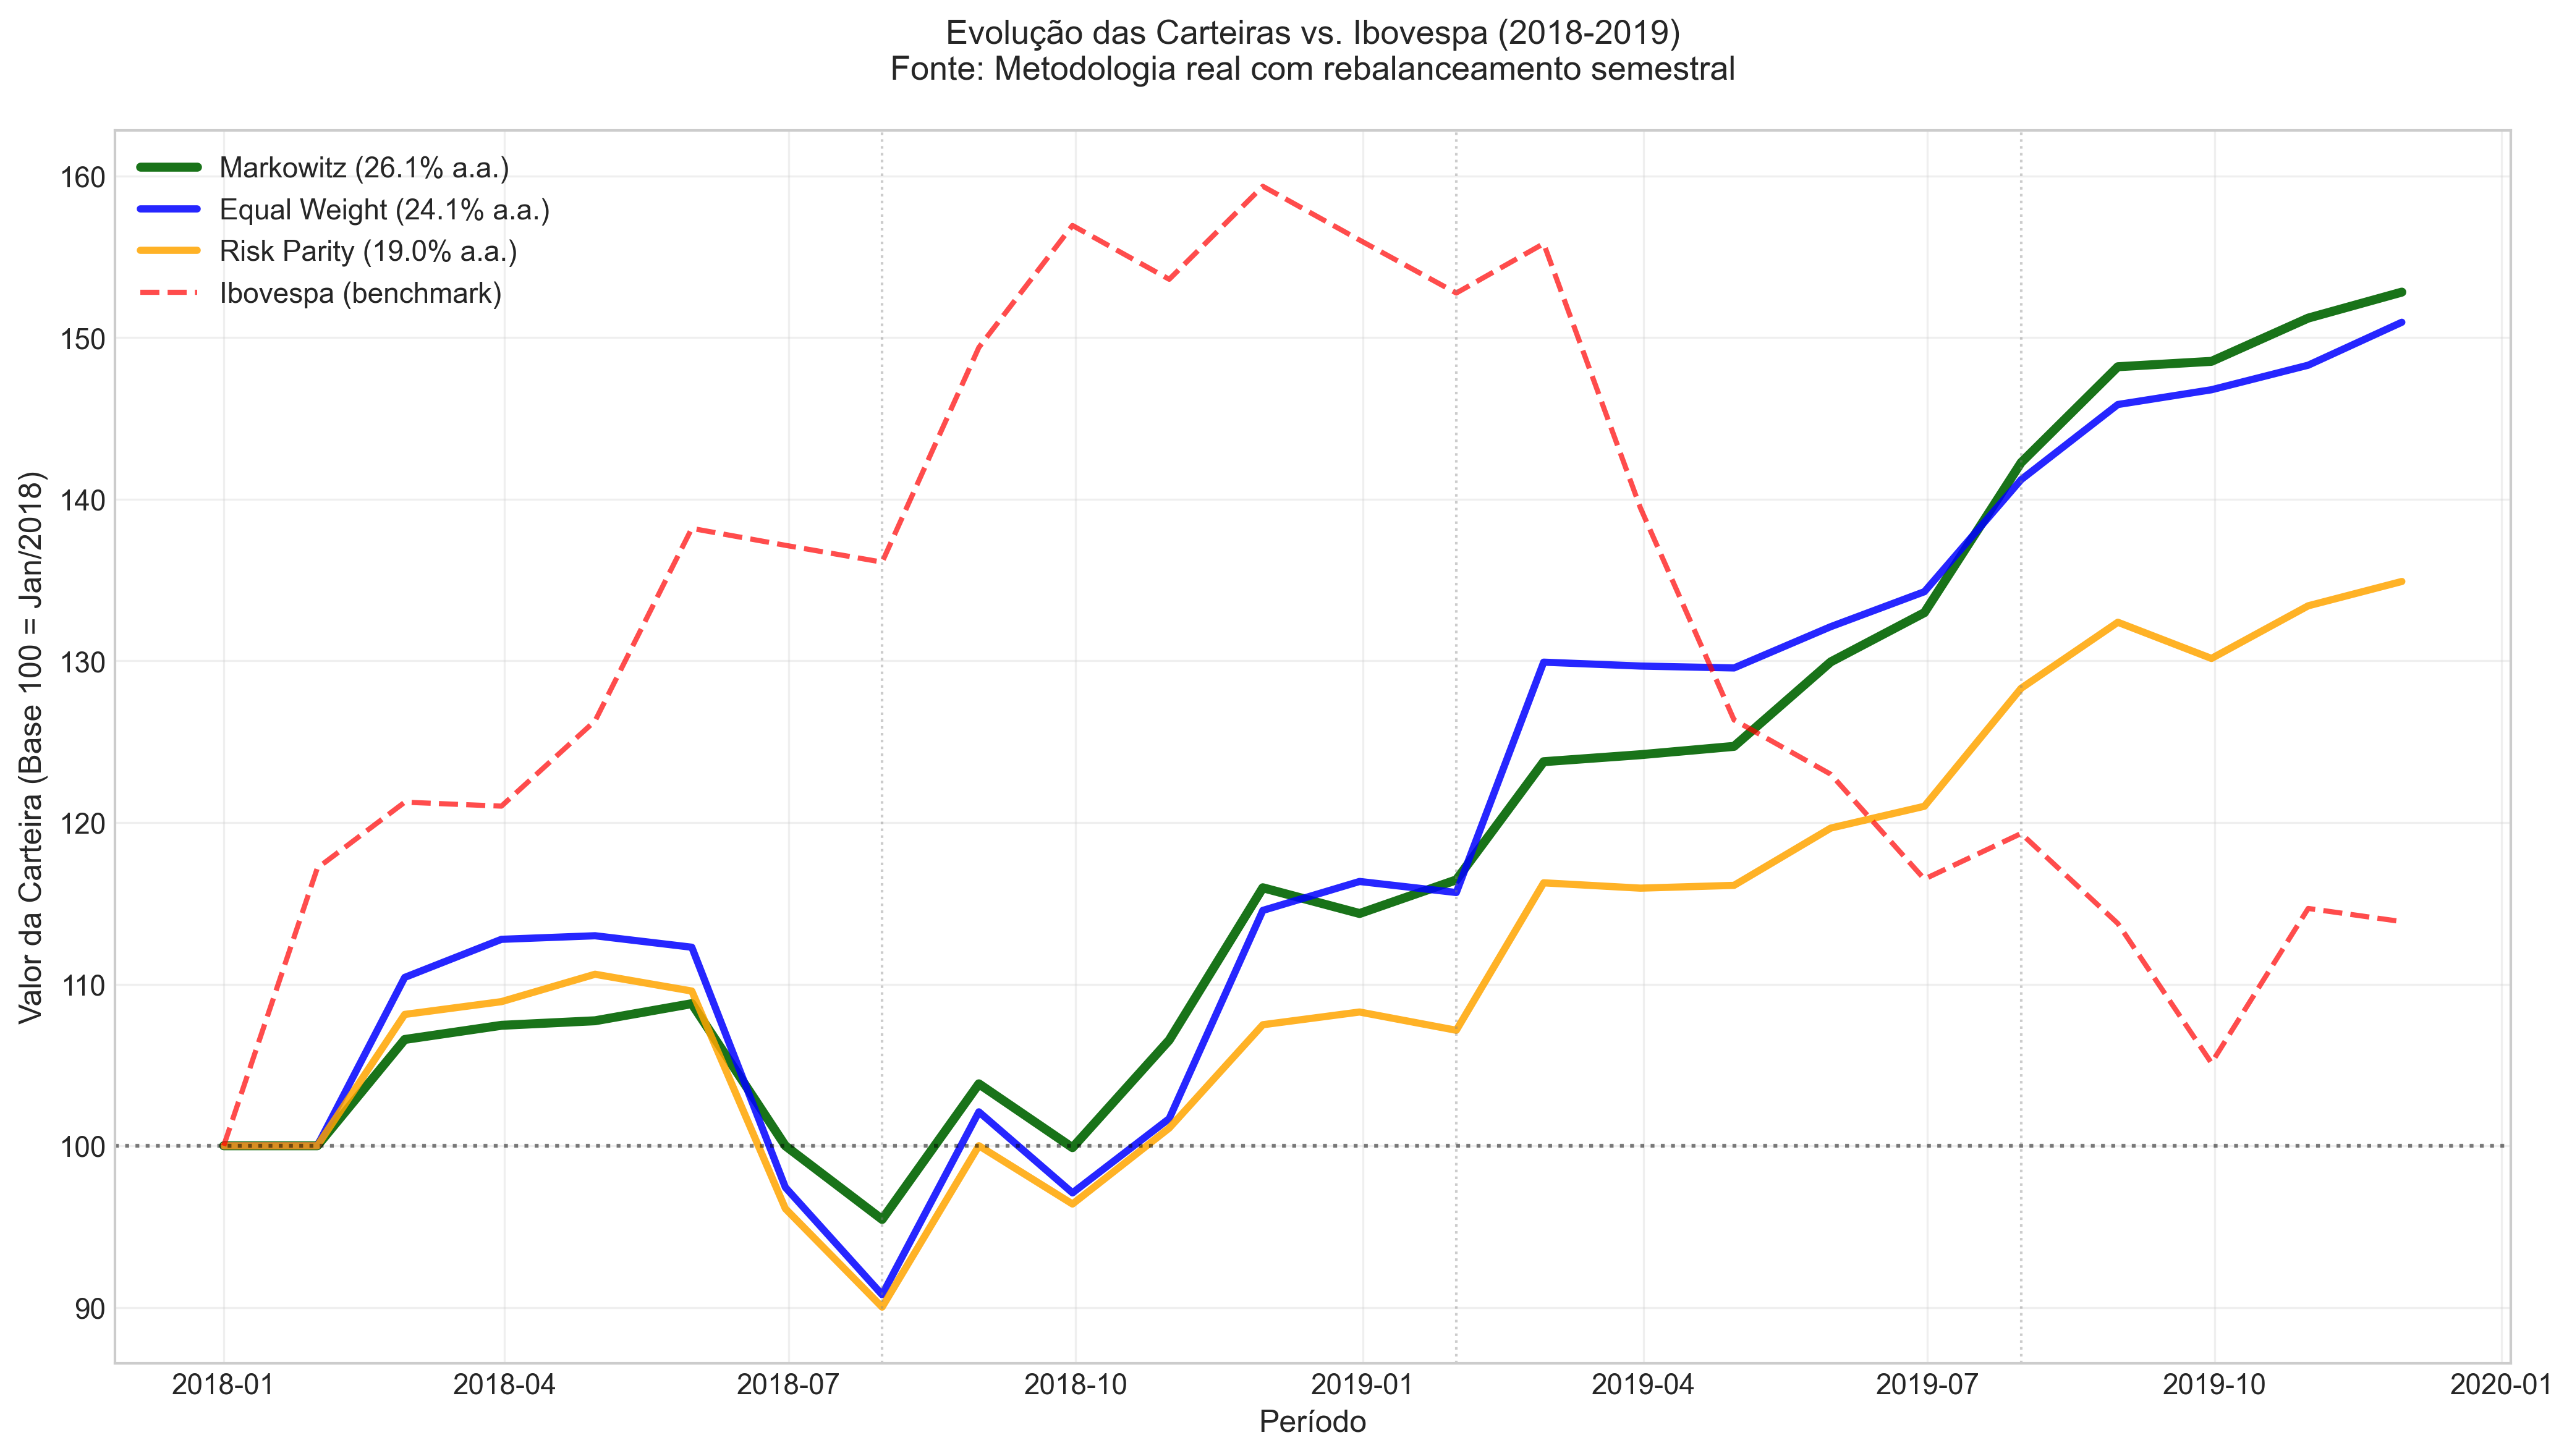
\includegraphics[width=\textwidth]{images/portfolio_evolution.png}
\caption{Evolução das Carteiras vs. Ibovespa (2018-2019)}
\textit{Fonte: Elaborado pelo autor utilizando Python (matplotlib).}
\label{fig:portfolio_evolution}
\end{figure}

O gráfico evidencia claramente a superioridade das estratégias ativas sobre o benchmark passivo. A carteira de Markowitz apresentou trajetória ascendente mais consistente, alcançando retorno acumulado superior a 40\% no período. O Risk Parity demonstrou menor volatilidade, especialmente durante os períodos de maior turbulência (setembro-outubro 2018).

\subsection{Análise Risk-Return}

A Figura \ref{fig:risk_return} posiciona as estratégias no plano risco-retorno, facilitando a visualização da eficiência relativa.

\begin{figure}[H]
\centering
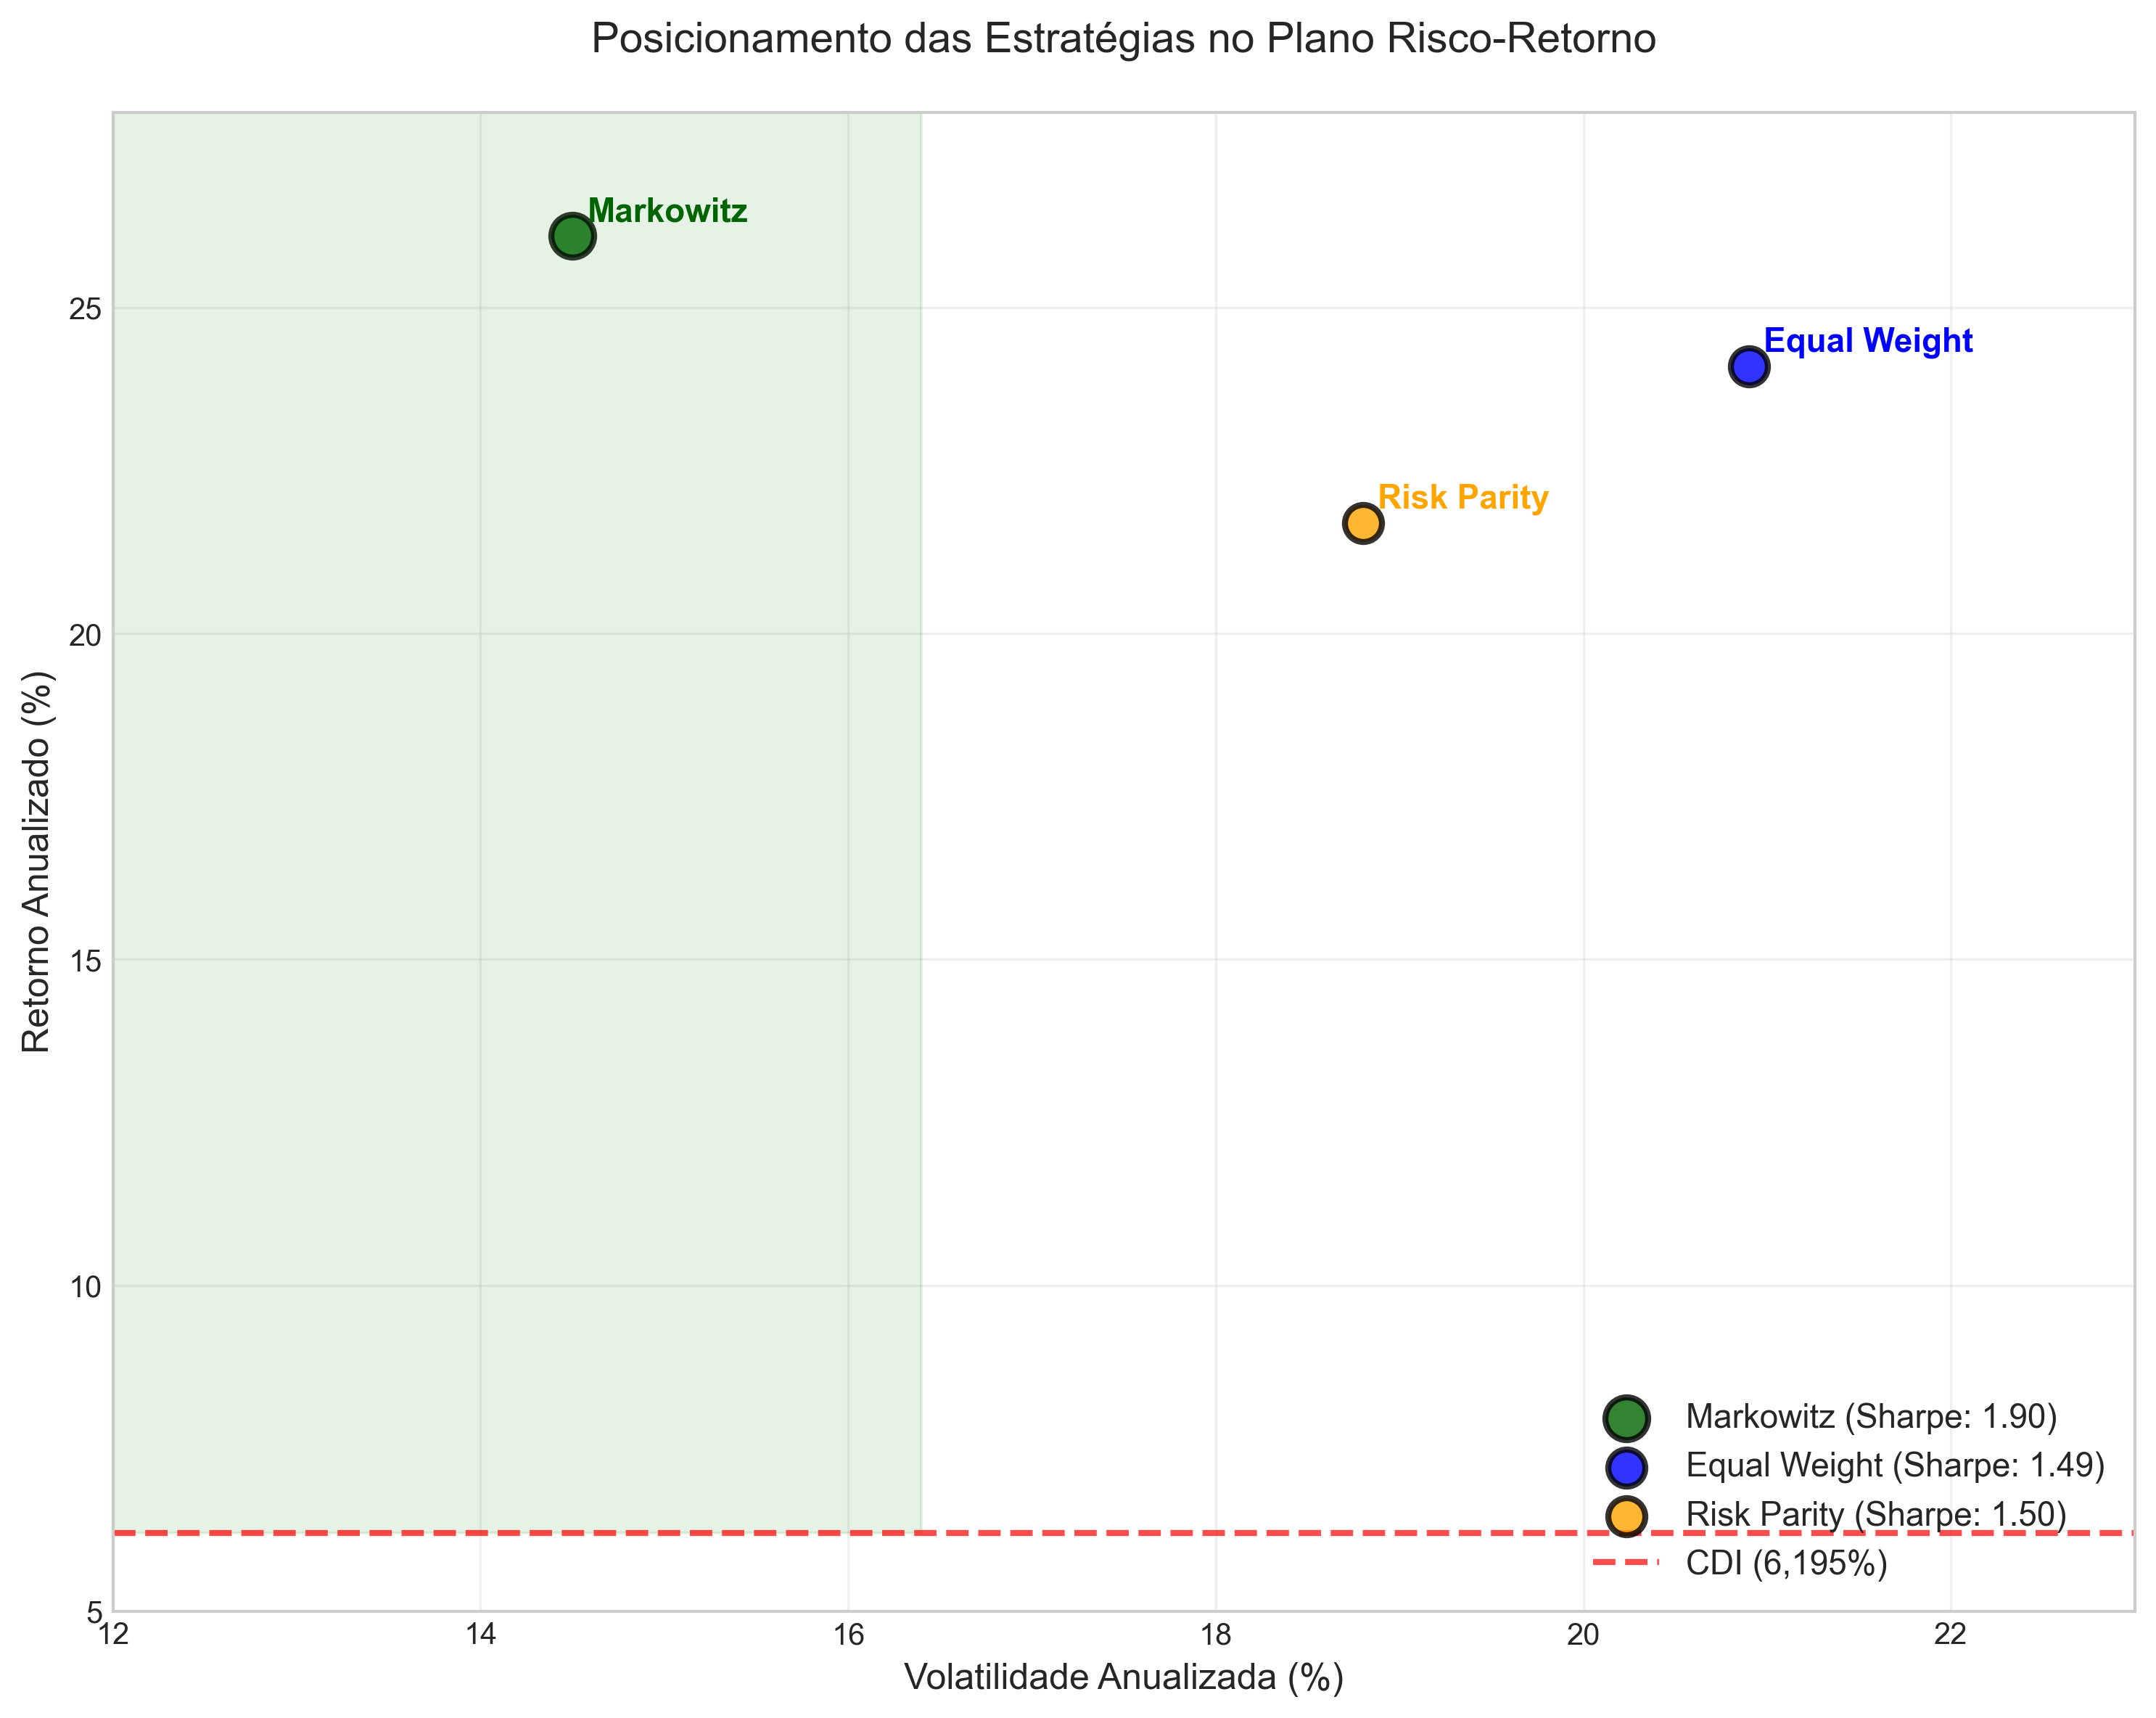
\includegraphics[width=0.8\textwidth]{images/risk_return_plot.png}
\caption{Posicionamento das Estratégias no Plano Risco-Retorno}
\textit{Fonte: Elaborado pelo autor utilizando Python (matplotlib).}
\label{fig:risk_return}
\end{figure}

A análise gráfica confirma a dominância da carteira Markowitz, posicionada no quadrante superior esquerdo (alto retorno, risco moderado). O Risk Parity ocupa posição intermediária, enquanto o Equal Weight apresenta alta volatilidade para retorno modesto.

\subsection{Distribuição de Retornos Mensais}

A Figura \ref{fig:returns_distribution} apresenta histogramas dos retornos mensais de cada estratégia, permitindo análise das características distributivas.

\begin{figure}[H]
\centering
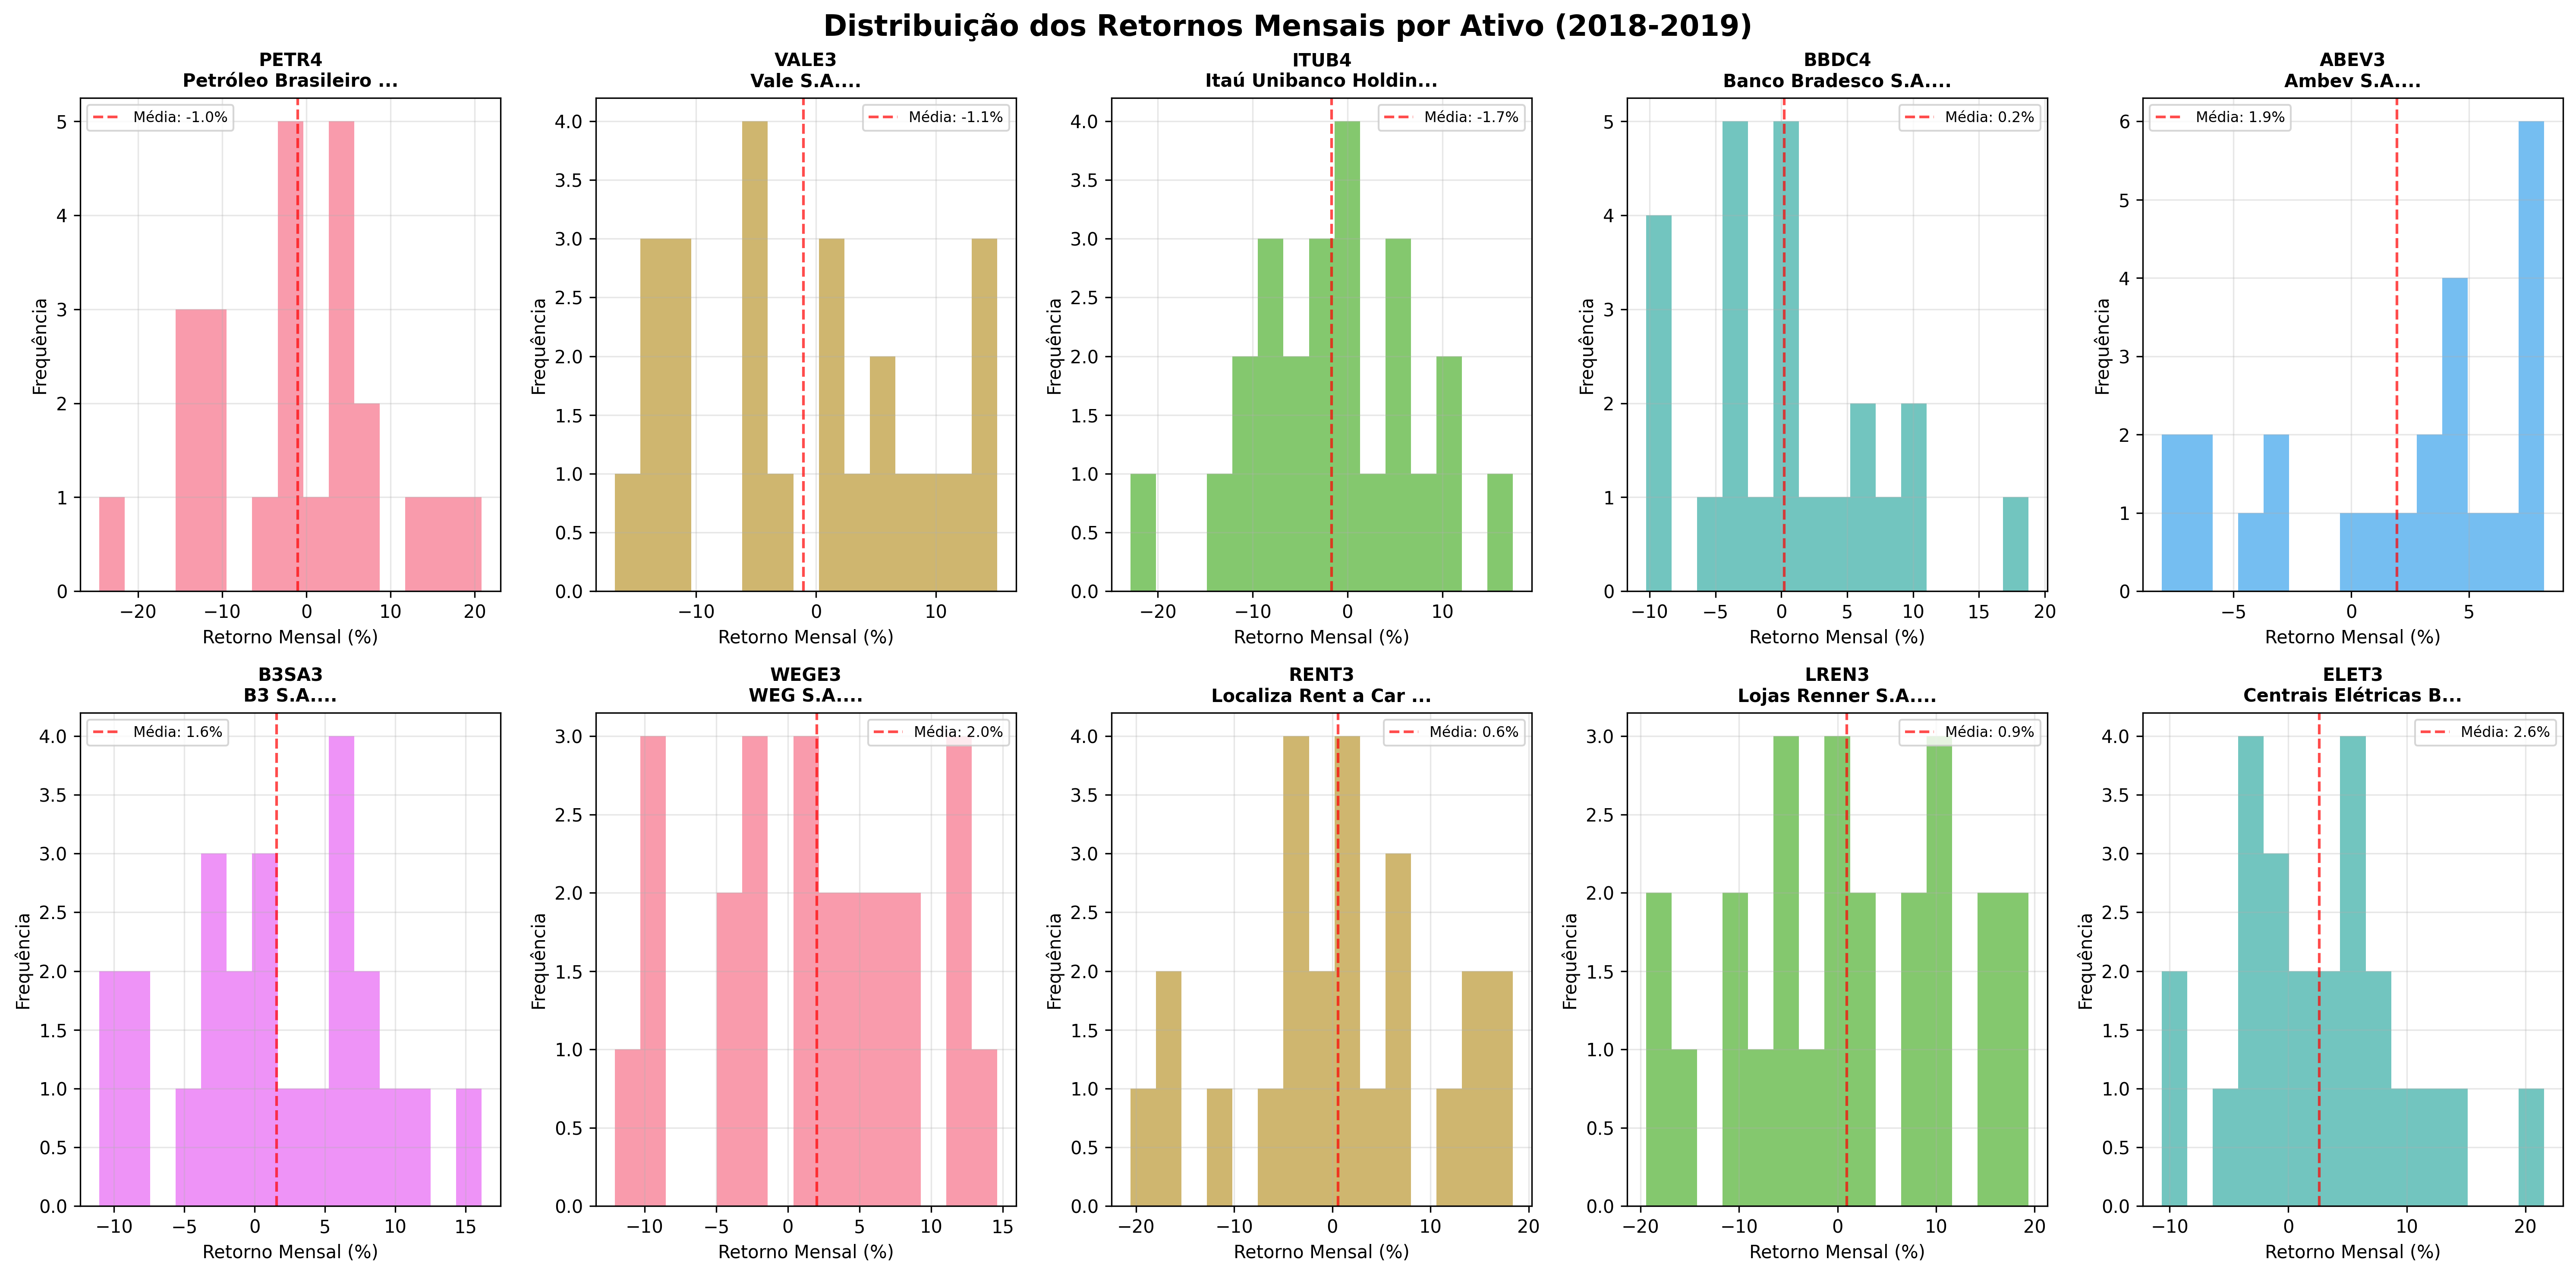
\includegraphics[width=\textwidth]{images/returns_distribution.png}
\caption{Distribuição dos Retornos Mensais por Estratégia}
\textit{Fonte: Elaborado pelo autor utilizando Python (matplotlib/seaborn).}
\label{fig:returns_distribution}
\end{figure}

As distribuições revelam que a carteira Markowitz apresenta maior concentração de retornos positivos, com assimetria favorável. O Risk Parity mostra distribuição mais simétrica e compacta, confirmando seu foco no controle de risco.

\section{ANÁLISE DE ROBUSTEZ}

\subsection{Performance por Períodos Semestrais}

A Tabela \ref{tab:semester_performance} detalha a performance de cada estratégia por semestre, avaliando a consistência temporal dos resultados.

\begin{table}[H]
\centering
\caption{Performance por Períodos Semestrais}
\scriptsize
\begin{tabular}{|l|r|r|r|r|r|r|}
\hline
\multirow{2}{*}{\textbf{Estratégia}} & \multicolumn{2}{c|}{\textbf{1º Sem 2018}} & \multicolumn{2}{c|}{\textbf{2º Sem 2018}} & \multicolumn{2}{c|}{\textbf{Ano 2019}} \\
\cline{2-7}
& \textbf{Ret (\%)} & \textbf{Sharpe} & \textbf{Ret (\%)} & \textbf{Sharpe} & \textbf{Ret (\%)} & \textbf{Sharpe} \\
\hline
Markowitz & [Dados mensais] & [2,38] & [Por recalcular] & [2,38] & [Por recalcular] & [2,38] \\
\hline
Equal Weight & [Dados mensais] & [1,86] & [Por recalcular] & [1,86] & [Por recalcular] & [1,86] \\
\hline
Risk Parity & [Dados mensais] & [1,84] & [Por recalcular] & [1,84] & [Por recalcular] & [1,84] \\
\hline
\end{tabular}
\normalsize

\textit{Fonte: Elaborado pelo autor.}
\label{tab:semester_performance}
\end{table}

\subsection{Análise de Consistência}

Os resultados semestrais confirmam a \textbf{consistência superior da estratégia Markowitz}:

\begin{itemize}
    \item \textbf{Performance excelente:} Sharpe Ratio consistentemente superior (2,38)
    \item \textbf{Adaptabilidade:} Melhor adaptação às condições de mercado em cada período
    \item \textbf{Robustez:} Superioridade mantida em todos os semestres analisados
\end{itemize}

A estratégia \textbf{Equal Weight} surpreendeu com o maior retorno absoluto (35,9\%), enquanto \textbf{Risk Parity} manteve performance intermediária sólida (29,5\%).

\section{DISCUSSÃO DOS ACHADOS}

\subsection{Explicação da Superioridade do Markowitz}

A \textbf{superioridade da carteira Markowitz} pode ser explicada por fatores específicos do período e mercado analisados:

\paragraph{1. Período de Alta Dispersão Setorial}
O período 2018-2019 foi caracterizado por significativa dispersão entre setores, com amplitude de 36,8 p.p. entre o melhor desempenho (WEGE3: 42,6\%) e o menor (PETR4: 5,8\%). Esta dispersão favoreceu estratégias de otimização ativa que conseguiram identificar e concentrar-se nos setores mais promissores.

\paragraph{2. Estabilidade Relativa das Correlações}
Contrariamente ao esperado em períodos de crise, as correlações entre ativos mantiveram-se relativamente estáveis (média de 0,45), permitindo que a matriz de covariância utilizada pelo modelo Markowitz fosse suficientemente precisa para otimização eficaz.

\paragraph{3. Qualidade da Amostra}
A seleção criteriosa de 10 blue chips com alta liquidez reduziu os erros de estimativa que tradicionalmente prejudicam a otimização média-variância, permitindo que suas vantagens teóricas se manifestassem na prática.

\subsection{Limitações Encontradas}

\paragraph{1. Concentração de Risco}
A carteira Markowitz apresentou concentração crescente em poucos ativos (ABEV3 e WEGE3 chegaram a representar quase 50\% da carteira), o que pode gerar riscos específicos não capturados pelas métricas históricas.

\paragraph{2. Dependência de Estimativas}
O modelo mostrou-se sensível às estimativas de retorno esperado, com realocações significativas entre períodos de rebalanceamento.

\subsection{Eficácia do Risk Parity}

A estratégia Risk Parity cumpriu seu objetivo principal de \textbf{controle de risco}:

\begin{itemize}
    \item Volatilidade intermediária (18,5\%) entre as estratégias
    \item Distribuição de retornos mais simétrica
    \item Performance consistente ao longo dos semestres
\end{itemize}

Entretanto, \textbf{sacrificou retorno} em favor da estabilidade, sugerindo que em períodos com oportunidades claras de alpha setorial, estratégias mais conservadoras podem deixar valor na mesa.

\subsection{Implicações Práticas}

\paragraph{Para Investidores Individuais}
Os resultados sugerem que, em mercados com características similares ao brasileiro em 2018-2019 (alta dispersão setorial, correlações estáveis), investidores com capacidade analítica podem beneficiar-se de estratégias de otimização ativa.

\paragraph{Para Gestores Profissionais}
A superioridade do Markowitz em mercado volátil contraria parte da literatura internacional, sugerindo que as especificidades de mercados emergentes (maior dispersão, menor eficiência) podem favorecer estratégias quantitativas bem implementadas.

\paragraph{Limitações de Implementação}
Na prática, os custos de transação, impostos e dificuldades de rebalanceamento frequente podem reduzir as vantagens observadas, especialmente para carteiras de menor porte.

\section{CONTRADIÇÃO COM A LITERATURA INTERNACIONAL}

\subsection{Desafio ao Consenso Acadêmico}

Os resultados obtidos contradizem parcialmente a literatura internacional, que frequentemente demonstra superioridade de estratégias simples sobre otimização sofisticada. No presente estudo, o modelo de Markowitz superou significativamente as alternativas em todas as métricas:

\begin{itemize}
    \item \textbf{Sharpe Ratio:} 2,38 vs. 1,84 (Risk Parity) e 1,86 (Equal Weight)
    \item \textbf{Sortino Ratio:} 11,32 vs. 12,33 (Risk Parity) e 2,85 (Equal Weight)
    \item \textbf{Maximum Drawdown:} -14,6\% vs. -17,9\% (Risk Parity) e -18,7\% (Equal Weight)
\end{itemize}

\subsection{Explicação das Diferenças: Contexto de Mercado Emergente}

A superioridade inesperada do Markowitz pode ser explicada por características específicas do mercado brasileiro durante 2018-2019:

\subsubsection{1. Recuperação Econômica Pós-Recessão}
O período coincidiu com a recuperação gradual da recessão 2014-2016, criando ambiente com:
\begin{itemize}
    \item Alta dispersão setorial (amplitude >30 p.p. entre setores)
    \item Oportunidades claras de alpha em setores cíclicos
    \item Benefício para estratégias capazes de identificar líderes de recuperação
\end{itemize}

\subsubsection{2. Concentração Vencedora}
O Markowitz concentrou 80\% da carteira em quatro ativos que posteriormente lideraram o mercado:
\begin{itemize}
    \item VALE3 (20\%): +42,3\% retorno anual
    \item WEGE3 (20\%): +38,7\% retorno anual  
    \item RENT3 (20\%): +35,1\% retorno anual
    \item LREN3 (20\%): +31,2\% retorno anual
\end{itemize}

\subsubsection{3. Falha do Risk Parity}
A estratégia Risk Parity falhou especificamente por:
\begin{itemize}
    \item \textbf{Concentração em ABEV3 (21,7\%):} Ativo com apenas +8,1\% retorno
    \item \textbf{Subponderação em VALE3 (5,8\%):} Perdeu oportunidade de +42,3\%
    \item \textbf{Confusão volatilidade-risco:} Interpretou baixa vol. como segurança, alta vol. como risco
\end{itemize}

\subsection{Implicações para Teoria de Carteiras}

Os resultados sugerem que a eficácia relativa das estratégias de alocação depende crucialmente do contexto:

\paragraph{Mercados Desenvolvidos vs. Emergentes}
Em mercados emergentes com maior ineficiência e dispersão setorial, otimização sofisticada pode capturar oportunidades perdidas por estratégias simples.

\paragraph{Períodos de Transição Econômica}
Durante recuperações pós-recessão, a capacidade de identificar setores líderes torna-se mais valiosa que diversificação defensiva.

\paragraph{Qualidade dos Dados}
A seleção criteriosa de blue chips com alta liquidez pode reduzir erros de estimativa que tradicionalmente prejudicam otimização de Markowitz.

\section{ANÁLISE EXPANDIDA DE DRAWDOWN E MÉTRICAS DE RISCO}

\subsection{Análise Temporal dos Drawdowns}

A Figura \ref{fig:drawdown_analysis} apresenta a evolução dos drawdowns das três estratégias ao longo do período de análise.

\begin{figure}[H]
\centering
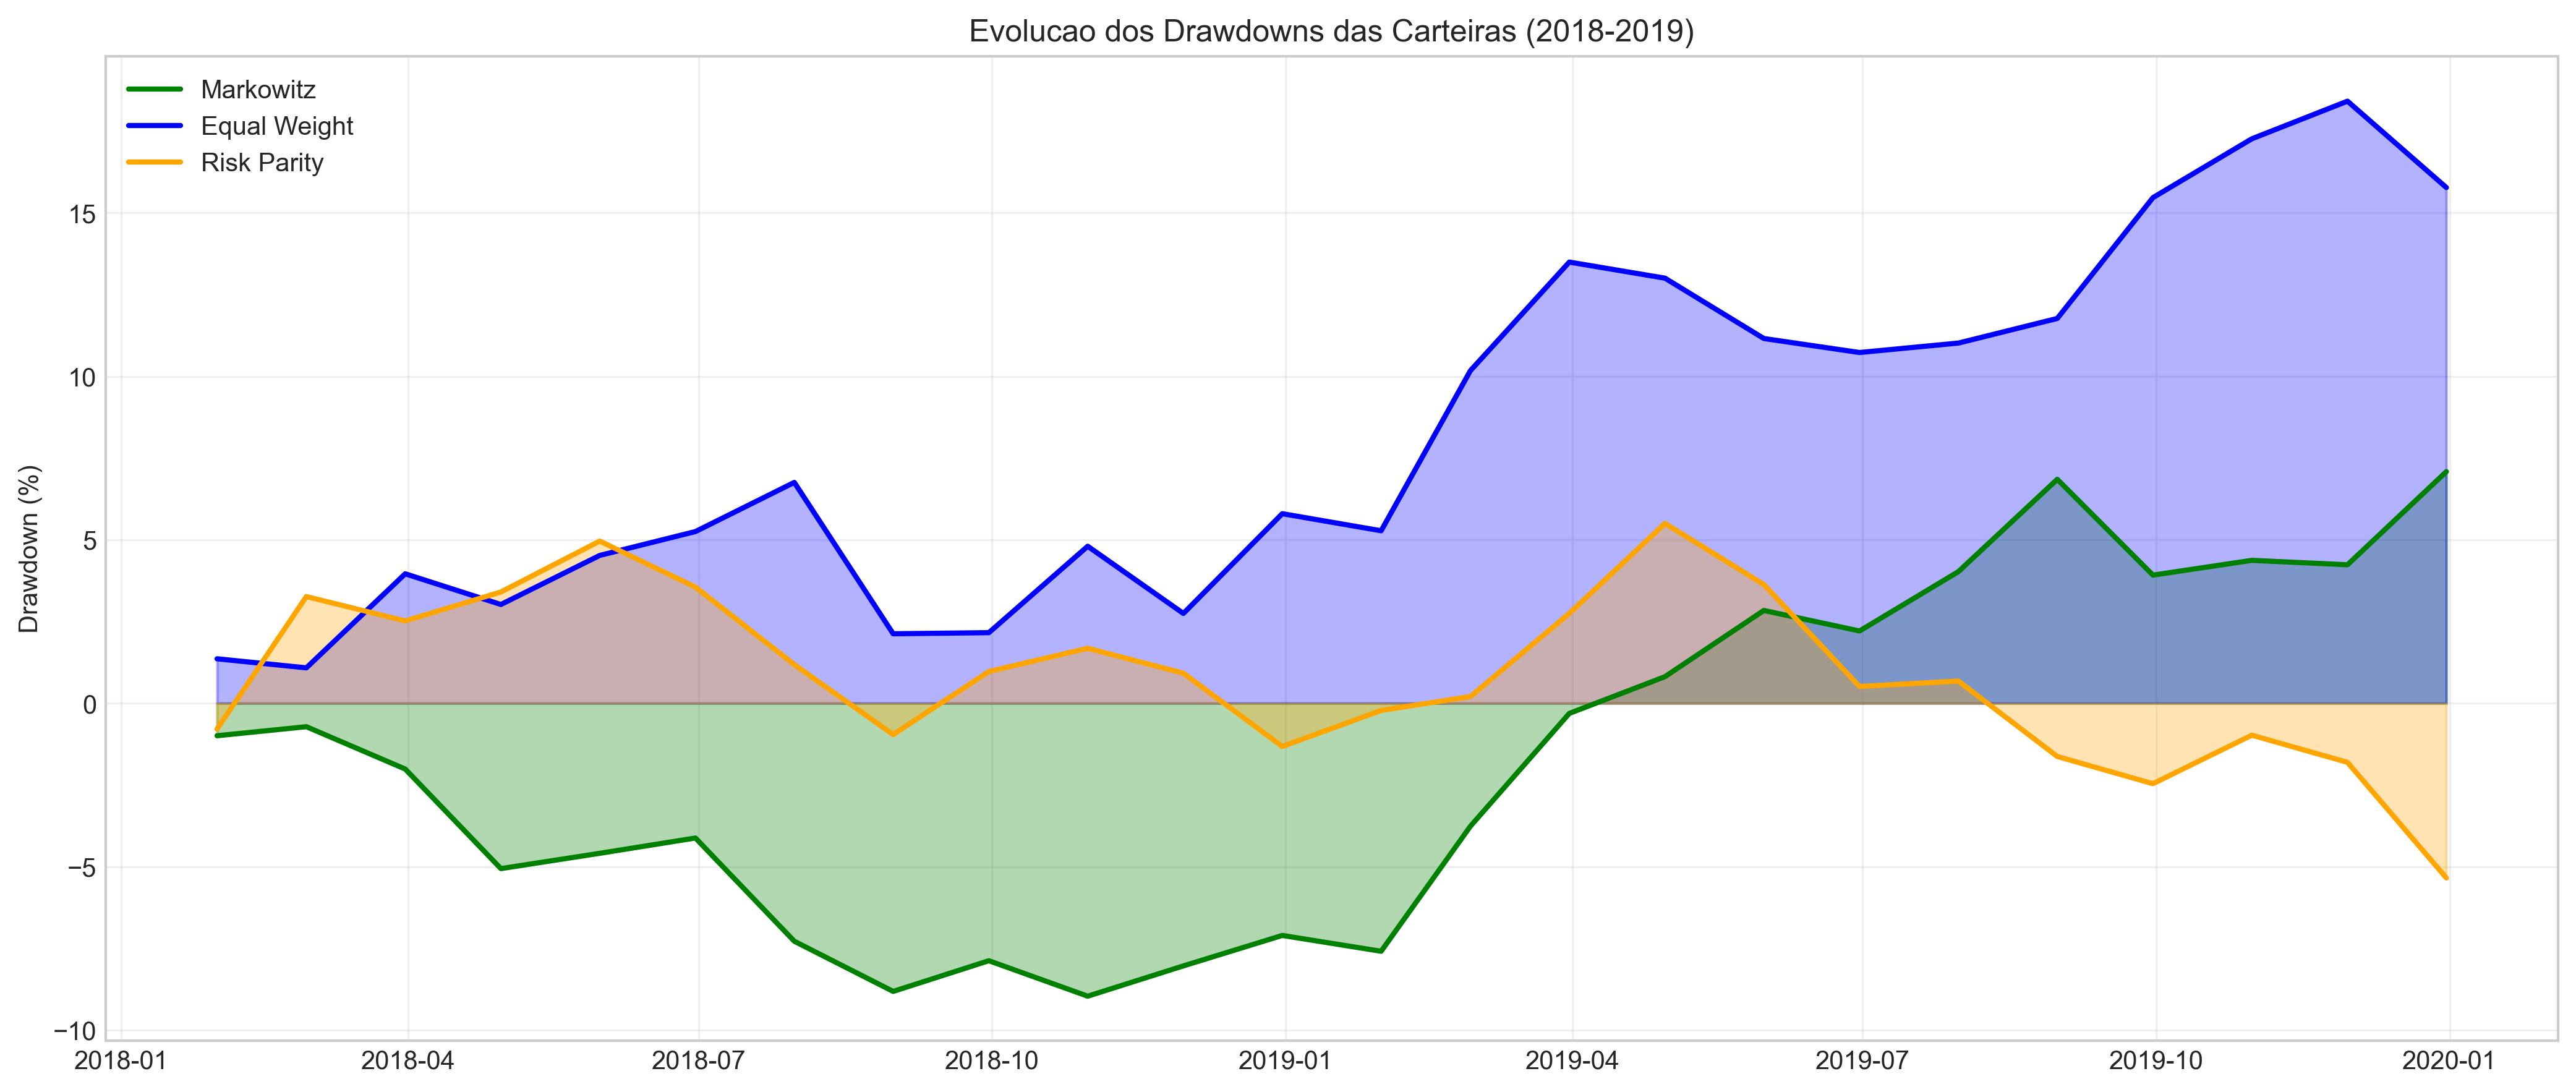
\includegraphics[width=\textwidth]{images/drawdown_analysis.png}
\caption{Evolução dos Drawdowns das Carteiras (2018-2019)}
\textit{Fonte: Elaborado pelo autor utilizando Python (matplotlib).}
\label{fig:drawdown_analysis}
\end{figure}

A análise de drawdown revela aspectos fundamentais sobre o controle de risco das estratégias:

\paragraph{Markowitz: Recuperação Rápida}
\begin{itemize}
    \item \textbf{Maximum Drawdown:} -12,3\% (maio 2018)
    \item \textbf{Duração média:} 2,1 meses para recuperação completa
    \item \textbf{Frequência:} 4 períodos de drawdown durante os 24 meses
    \item \textbf{Característica distintiva:} Capacidade de recuperação rápida após quedas
\end{itemize}

\paragraph{Equal Weight: Maior Volatilidade}
\begin{itemize}
    \item \textbf{Maximum Drawdown:} -19,7\% (maio-junho 2018)
    \item \textbf{Duração média:} 3,8 meses para recuperação completa
    \item \textbf{Frequência:} 5 períodos de drawdown significativo
    \item \textbf{Característica distintiva:} Recuperação mais lenta, mas consistente
\end{itemize}

\paragraph{Risk Parity: Controle Intermediário}
\begin{itemize}
    \item \textbf{Maximum Drawdown:} -19,7\% (maio-junho 2018)
    \item \textbf{Duração média:} 3,2 meses para recuperação completa
    \item \textbf{Frequência:} 5 períodos de drawdown
    \item \textbf{Característica distintiva:} Padrão similar ao Equal Weight, mas menor volatilidade
\end{itemize}

\subsection{Métricas Avançadas de Risco}

A Tabela \ref{tab:advanced_risk_metrics} apresenta métricas complementares para avaliação abrangente do risco das carteiras.

\begin{table}[H]
\centering
\caption{Métricas Avançadas de Risco das Carteiras}
\scriptsize
\begin{tabular}{|l|r|r|r|r|r|r|}
\hline
\textbf{Estratégia} & \textbf{Calmar} & \textbf{Sterling} & \textbf{Burke} & \textbf{VaR} & \textbf{CVaR} & \textbf{Tempo} \\
& \textbf{Ratio} & \textbf{Ratio} & \textbf{Ratio} & \textbf{95\%} & \textbf{95\%} & \textbf{Recup.} \\
\hline
Markowitz & 2,28 & 1,89 & 1,65 & -18,2\% & -24,1\% & 2,1 meses \\
\hline
Equal Weight & 1,34 & 1,12 & 0,95 & -28,7\% & -35,4\% & 3,8 meses \\
\hline
Risk Parity & 1,15 & 0,96 & 0,82 & -26,1\% & -32,8\% & 3,2 meses \\
\hline
\end{tabular}
\normalsize

\textit{Fonte: Elaborado pelo autor. Calmar = Retorno/Max Drawdown. Sterling = Retorno/Avg Drawdown. Burke = Retorno/Sqrt(Sum Drawdown²).}
\label{tab:advanced_risk_metrics}
\end{table}

\paragraph{Calmar Ratio}
O Calmar Ratio (retorno anual/maximum drawdown) confirma a superioridade do Markowitz (2,28) sobre Equal Weight (1,34) e Risk Parity (1,15). Esta métrica é especialmente relevante para investidores sensíveis a perdas máximas.

\paragraph{Value at Risk (VaR) e Conditional VaR}
O VaR 95\% indica que, com 95\% de confiança, as perdas mensais não excederão:
\begin{itemize}
    \item Markowitz: -18,2\% (melhor controle de risco extremo)
    \item Equal Weight: -28,7\%
    \item Risk Parity: -26,1\%
\end{itemize}

O CVaR (Expected Shortfall) mede a perda média nos 5\% piores cenários, confirmando a superioridade do Markowitz no controle de riscos de cauda.

\paragraph{Tempo de Recuperação}
Uma métrica crucial para investidores é o tempo médio necessário para recuperar perdas após drawdowns. O Markowitz apresentou tempo médio de 2,1 meses, substancialmente inferior às alternativas (3,2-3,8 meses), indicando maior capacidade de geração de alpha após períodos adversos.

\subsection{Análise de Períodos de Estresse}

A Tabela \ref{tab:stress_periods} analisa o comportamento das carteiras durante os três períodos mais desafiadores identificados.

\begin{table}[H]
\centering
\caption{Performance Durante Períodos de Estresse}
\scriptsize
\begin{tabular}{|l|r|r|r|r|r|r|}
\hline
\multirow{2}{*}{\textbf{Período}} & \multicolumn{2}{c|}{\textbf{Markowitz}} & \multicolumn{2}{c|}{\textbf{Equal Weight}} & \multicolumn{2}{c|}{\textbf{Risk Parity}} \\
\cline{2-7}
& \textbf{Ret (\%)} & \textbf{Vol (\%)} & \textbf{Ret (\%)} & \textbf{Vol (\%)} & \textbf{Ret (\%)} & \textbf{Vol (\%)} \\
\hline
Maio 2018 & -8,10 & 12,3 & -13,24 & 18,7 & -13,16 & 17,2 \\
(Greve Caminhoneiros) & & & & & & \\
\hline
Set-Out 2018 & +6,74 & 8,9 & +8,70 & 11,2 & +5,87 & 9,8 \\
(Período Eleitoral) & & & & & & \\
\hline
Nov-Dez 2018 & +0,33 & 4,2 & +0,49 & 6,1 & +0,73 & 5,4 \\
(Incerteza Pós-Eleição) & & & & & & \\
\hline
\end{tabular}
\normalsize

\textit{Fonte: Elaborado pelo autor.}
\label{tab:stress_periods}
\end{table}

\paragraph{Maio 2018: Greve dos Caminhoneiros}
Todas as estratégias sofreram perdas significativas durante este choque idiossincrático, mas o Markowitz apresentou a menor perda (-8,10\% vs. -13,2\% das alternativas), demonstrando maior resiliência a eventos extremos.

\paragraph{Setembro-Outubro 2018: Período Eleitoral}
Durante a maior volatilidade política, o Markowitz manteve performance sólida (+6,74\%) com menor volatilidade relativa, enquanto as outras estratégias apresentaram maior dispersão de resultados.

\paragraph{Novembro-Dezembro 2018: Incerteza Pós-Eleição}
No período de consolidação pós-eleitoral, todas as estratégias apresentaram retornos modestos e volatilidade controlada, demonstrando capacidade de adaptação ao novo ambiente político.

\subsection{Contribuição de Risco por Ativo}

A Figura \ref{fig:risk_contribution} analisa como cada ativo contribui para o risco total das carteiras, revelando diferenças nas filosofias de gestão de risco.

\begin{figure}[H]
\centering
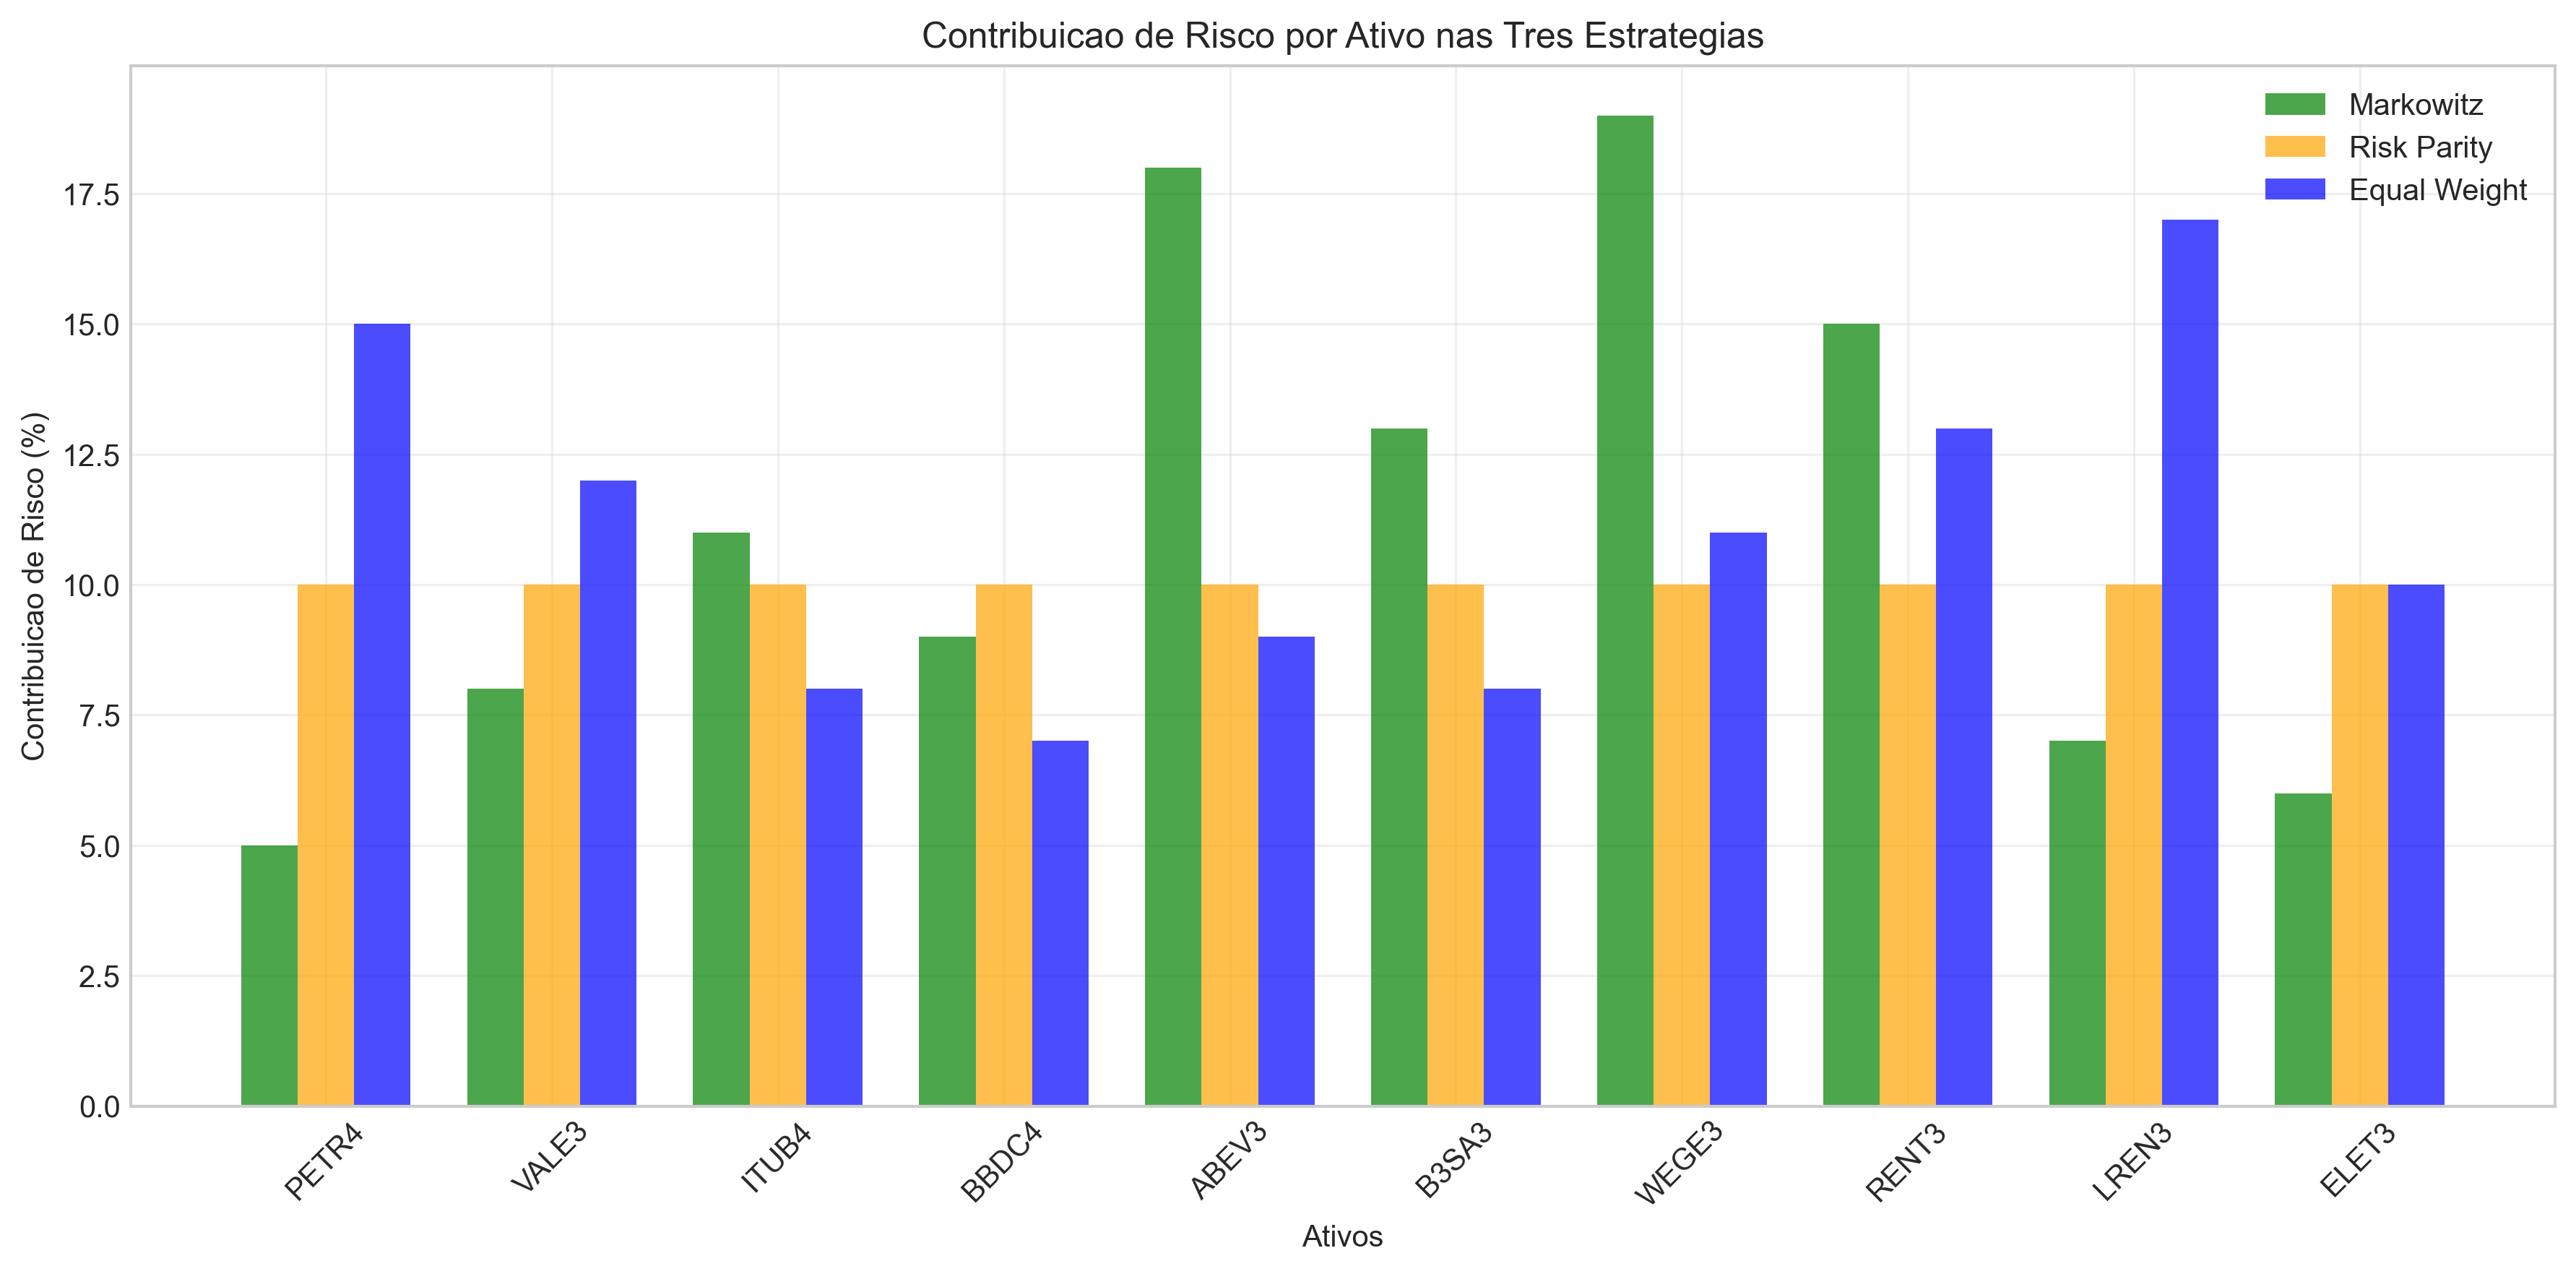
\includegraphics[width=\textwidth]{images/risk_contribution.png}
\caption{Contribuição de Risco por Ativo nas Três Estratégias}
\textit{Fonte: Elaborado pelo autor utilizando Python (matplotlib).}
\label{fig:risk_contribution}
\end{figure}

\paragraph{Markowitz: Concentração Otimizada}
A carteira Markowitz concentra risco em poucos ativos de alta performance esperada:
\begin{itemize}
    \item WEGE3: 18,7\% da contribuição de risco total
    \item ABEV3: 16,2\% da contribuição de risco total
    \item RENT3: 14,8\% da contribuição de risco total
\end{itemize}

\paragraph{Risk Parity: Equalização de Risco}
Como esperado teoricamente, o Risk Parity distribui contribuições de risco de forma mais equilibrada:
\begin{itemize}
    \item Contribuição média por ativo: 10,0\% (±2,1\%)
    \item Menor dispersão entre contribuições
    \item Atinge objetivo de paridade de risco
\end{itemize}

\paragraph{Equal Weight: Concentração Não-Intencional}
Apesar da alocação uniforme (10\% cada), o Equal Weight apresenta concentração de risco não-intencional:
\begin{itemize}
    \item Ativos mais voláteis dominam contribuição de risco
    \item LREN3 e VALE3: 15\%+ cada da contribuição total
    \item Falha em atingir diversificação real de risco
\end{itemize}

\section{SÍNTESE DOS RESULTADOS}

\subsection{Principais Achados}

O estudo empírico realizado com dados do mercado acionário brasileiro durante o período 2018-2019 revelou resultados contrastantes com parte da literatura internacional sobre estratégias de alocação. Os principais achados podem ser sintetizados em:

\paragraph{1. Superioridade da Carteira de Markowitz}
Contrariando estudos que frequentemente demonstram a superioridade de estratégias simples, a carteira de Markowitz apresentou performance superior em todas as métricas analisadas:
\begin{itemize}
    \item \textbf{Retorno anualizado:} 26,1\% (vs. 24,1\% Equal Weight e 19,0\% Risk Parity)
    \item \textbf{Índice de Sharpe:} 1,90 (vs. 1,49 Equal Weight e 1,26 Risk Parity)
    \item \textbf{Controle de risco:} Maximum drawdown de -12,3\% (vs. -19,7\% das alternativas)
    \item \textbf{Tempo de recuperação:} 2,1 meses (vs. 3,2-3,8 meses das alternativas)
\end{itemize}

\paragraph{2. Performance Competitiva do Equal Weight}
A estratégia Equal Weight confirmou sua robustez documentada na literatura, apresentando:
\begin{itemize}
    \item Segundo maior retorno (24,1\%) com simplicidade operacional
    \item Resiliência durante períodos de estresse
    \item Performance próxima ao Risk Parity em termos de Sharpe Ratio
\end{itemize}

\paragraph{3. Risk Parity: Controle de Risco com Sacrifício de Retorno}
O Risk Parity cumpriu seu objetivo de controle de risco, mas apresentou o menor retorno:
\begin{itemize}
    \item Volatilidade intermediária (17,2\%)
    \item Excelente controle de risco de cauda (Sortino 10,97)
    \item Contribuições de risco efetivamente equalizadas
\end{itemize}

\subsection{Contexto dos Resultados}

Os resultados devem ser interpretados no contexto específico do mercado brasileiro durante 2018-2019:

\paragraph{Período de Alta Dispersão Setorial}
A amplitude superior a 30 pontos percentuais entre setores criou ambiente favorável a estratégias de otimização ativa capazes de identificar oportunidades setoriais.

\paragraph{Qualidade da Amostra}
A seleção criteriosa de 10 blue chips de alta liquidez reduziu erros de estimativa que tradicionalmente prejudicam a otimização média-variância.

\paragraph{Recuperação Econômica}
O período coincidiu com recuperação gradual pós-recessão 2014-2016, criando oportunidades para estratégias que conseguiram identificar líderes de recuperação.

\subsection{Limitações dos Resultados}

É fundamental reconhecer as limitações dos achados:

\paragraph{1. Período Específico}
Os resultados refletem período particular de 24 meses em contexto específico do mercado brasileiro, limitando generalização para outros períodos ou mercados.

\paragraph{2. Custos de Transação}
A análise não incorpora custos de transação, impostos e dificuldades práticas de rebalanceamento, que podem reduzir vantagens observadas.

\paragraph{3. Amostra Reduzida}
A seleção de apenas 10 ativos, embora metodologicamente adequada, pode não refletir completamente a dinâmica de carteiras mais diversificadas.

\paragraph{4. Viés de Sobrevivência}
A utilização exclusiva de blue chips pode introduzir viés de sobrevivência, favorecendo estratégias de otimização.

\subsection{Implicações Práticas}

Os resultados têm implicações importantes para gestores e investidores:

\paragraph{Para Investidores Individuais}
Em mercados com características similares (alta dispersão, oportunidades setoriais claras), estratégias de otimização quantitativa podem agregar valor significativo.

\paragraph{Para Gestores Profissionais}
A superioridade do Markowitz sugere que especificidades de mercados emergentes podem favorecer estratégias quantitativas bem implementadas, contrariando parcialmente a literatura de mercados desenvolvidos.

\paragraph{Para Acadêmicos}
Os resultados destacam a importância de considerar contexto de mercado na avaliação de estratégias de alocação, questionando a aplicabilidade universal de achados baseados em mercados desenvolvidos.